%\documentclass[letter]{article}
\documentclass[letter,12pt]{article}
\usepackage[letterpaper,right=1in,left=1in,top=1in,bottom=1in]{geometry}

\usepackage{hyperref}
\usepackage{url}
\usepackage[pdftex]{graphicx}
\usepackage[longnamesfirst, sort]{natbib}\bibpunct[]{(}{)}{,}{a}{}{;}
\usepackage{arydshln}
\usepackage{amsmath}

\newcommand{\mc}{\multicolumn}

\begin{document}

\title{A preliminary inspection of recent \\ 
       redistricting proposals and the status quo}
\author{Eric Magar\\ITAM\\ {\small \url{emagar@itam.mx}}
      }
\date{\today}
\maketitle


\begin{abstract}
  \noindent Unlike analysis of the votes-to-seats conversion at the national-level, state-level data reveal no evidence of systematic party bias. What bias there is in federal districts is of another kind, a big bonus for larger parties (or vote responsiveness), typical of plurality rule in single-member districts. Since states disitribute relatively few seats each, the large party bonus of states' federal districts doubles the estimate with national data. Since the PRI is the large party in most states, it receives a substantial seat bonus.
\end{abstract}

Comentario FEE Gracias, Eric.  Interesante hallazgo a nivel de los estados y similar a los ejercicios analíticos (tú les dices contrafácticos) que varios hicimos entre 1997 y 2003.  Lo que nunca se ha hecho y tienes chance de hacer con estos datos es aislar mejor los mecanismos de distorsión, dada la tecnología del IFE.  Por ejemplo, la "discreción" con la que deciden los expertos sobre- o sub-poblar a los distritos dentro de todo estado ¿conlleva algo sesgo partidista sistemático?  ¿Cómo afecta "reapportionment" a los premios y castigos? (Recuerdo que la reducción de distritos en el DF para 2006 afectó al PAN negativamente, no tanto por el peso de la mayoría de la izquierda sino por las tendencias demográficas aceleradas en zonas panistas -- y también porque en la redistritación de 1997 se usaron "proyecciones" censales a final de cuentas exageradas, error técnico que igual y afecte en menor grado al plan de redistritación del año pasado.)  Seguro que existen otras fuentes de discreción o error convertibles en sesgo.  Trelles, en el pasado, ha avalado la relativa pureza del mole técnico del IFE, pero dudo que sostenga la misma posición hoy.  Por otra parte, la microinformación con la que cuenta el IFE hoy (que no tenía el IFE de 1996 ni el de 2003) permite evitar lo que señalas como posible injerencia partidista desde el principio en el proceso de dibujar los distritos (según Trelles, ahora es aleatoria la selección de los puntos de inicio de conformación   distrital).  Yo diría que el proceso de sugerencias y críticas por los partidos afectó, overall, muy poco al resultado -- aunque tampoco es poca cosa el 10 a 12\% de los distritos afectados en cuatro meses de revisión. También sospecho que los partidos durante el período de revisión emplearon distintas estrategias con distintas prioridades.  Bien puedo imaginar que todos buscaran proteger a sus bastiones, pero el PRI también tendría interés en maximizar sus distritos ganados.  El PAN y la izquierda, no tanto.  Por último, el análisis margina otro factor que Weldon siempre ha resaltado -- la presión ejercida por la burocracia distrital del IFE para no tener que mudarse de oficina y quizá hogar (en la versión de Jeff, los consejeros y vocales del IFE son quienes han sustituido a los incumbents en estos procesos de redistritación).  Cuestión de ver si cabeceras distritales cambian al rehacer la cartografía electoral.  En fin, para explicar cómo una redistritación hecha por expertos se desvía de lo ideal, debe juzgársele con criterios distintos a los aplicados a una hecha por políticos.  FEE

Eric, dado que la prueba de sesgos partidistas, si acaso, consistirá en una extrapolación de votos de la elección federal anterior, lo mejor sería nombrar a tus "estructuras" (¿por qué no hablas mejor de "cartografía distrital" o mapas distritales?) por su vigencia electoral en vez de legal, con referencia nominal solamente al primer año de elección federal en que se aplicó una nueva distritación.  Así:  1979, 1997, 2006, y 2015 prop.  Obviamente, los cambios más dramáticos se verían con la redistritación en 1997, si sólo por los sesgos originales de 1979 más el paso del tiempo.  Si crees que la dinámica poblacional inter-censal puede confundir al lector con la secuencia de redistritaciones, entonces puedes llamarlos:  1979 map, 1997 map, etc.  Aparte, la posible influencia de algún técnico o consejero disminuye en el tiempo.  Si recuerdo bien lo de Trelles, el mole empleado para el mapa de 2006 y la técnica semi-bayesiana de la propuesta de 2013  determinan, por ejemplo, el sesgo de sobre y subpoblación de los distritos, que puede mejorar o empeorar en el proceso de revisión, pero solamente en el margen.  Entonces, el grado de discreción ha disminuido, en balance.  Ni de chiste se impuso Morales como lo habían hecho el grupo de Reyes Heroles y el de Creel y Woldenberg (salvo con respecto a los criterios para diseñar distritos "indígenas", que en algo se parecen a los distritos gringos de representación de minorías).  El otro detalle tiene que ver con el peso de los estados subpoblados que tuviesen derecho a la mínima representación de dos distritos, número mucho más fuerte en 1979 que hoy.  No me refiero al problema de "apportionment", sino al problema secundario que ese reparto introduce al juego, dado que ambos distritos serán subpoblados pero no recuerdo criterio legal para asegurar equidad poblacional entre ellos.  Mayor margen de maniobra, pues, y sobre todo una vez que se introduce el criterio de no-división municipal (para 1997, creo).  Suerte, FEE

% La propuesta, o adopci\'on, de un plan redistritaci\'on viene acompa\~nada de una sospecha: que quien prepar\'o dicho plan haya 
% inclinado la balanza de la competencia en favor de unos y en contra de otros. Elaborar acerca del Gerrymandering. 

\noindent This note inspects IFE's recent federal redistricting proposal, the discussion and adoption of which has been postponed by the Council General until after the 2015 midterm election, in search for party effects. The focus of analysis are single-member district (SMD) seats in the federal chamber of deputies. The compensatory, proportional representation (PR) seats, untouched by the redistricting proposal, are removed from the picture. 

Investigation follows two routes. One is counterfactual analysis, asking how would votes have converted into seats in recent congressional elections had the redistricting proposal been used in stead of the actual ditricts. M\'arquez (\href{http://bit.ly/1nk4kYs}{\url{http://bit.ly/1nk4kYs}}) did this using national aggregates over two decades. I proceed with state-by-state breakdowns (over much a shorter span: 2006, 2009, and 2012), uncovering many seat changes that cancel out in the aggregate. Compared to actual districts, counterfactual districts would slightly benefit the PRI nationwide and, by alliance, the Green party, granting them 2 to 3 extra deputies; would slightly hurt the PAN, erasing 2 to 4 victories; and would, on average, leave the left unaffected. Analysis also reveals distributive effects in nearly half the states, which complicates the assessment of partisan effects of the redistricting proposal.

The other route estimates districts' responsivity and party bias --- two effects of scholarly interest, discussed below. M\'arquez (\href{http://bit.ly/1jgsQXE}{\url{http://bit.ly/1jgsQXE}}) has also approached this with national aggregates, uncovering a degree of responsivity characteristic of Westminster systems and party bias against the PAN under the status quo districts. By proceeding with state aggregates, much higher responsivity (owing to fewer districts, 9 by state on average) is uncovered, but no apparent party bias in neither actual nor proposed districts. 

Two redistricting proposals will be considered. One is the initial proposal prepared by IFE's specialists early in the redistricting process. This proposal met all the technical criteria but had not yet received input by the parties. The other is the final proposal that was submitted to IFE's Council General for approval. The third or final proposal includes two rounds of comments from the parties. Comparing these proposals should offer perspective to appreciate whether and how parties influence expert electoral regulation in general \citep{estevez.magar.rosas.2008}, and district line drawing in particular \citep{rossiter.etal.1997,cox.katz.2002}. 

\section{Winners and losers}

Counterfactuals are prepared with IFE's so-called ``scenarios'': the first scenario, presented on July 17, 2013 for discussion with party representatives; and the third, presented on October 15, 2013 for Council General approval. The first proposal had, presumably, anticipated key elements of party positions on redistricting, but had not been evaluated by parties directly. The third proposal includes party feedback, hundreds of direct requests, complaints, and counter-proposals made by party representatives in the technical committees to two preliminary proposals. (Alejandro, some descriptive of number of amendments?) 

%Two weeks later, the Council General decided to postpone the discussion and approval of new congressional districts (the 2015 midterm election, we later learned, will be held with outdated districts). 

Column $S$ of Tables \ref{T:2006}, \ref{T:2009}, and \ref{T:2012} breaks down the federal deputy seats that parties won in the last three congressional elections by state (with actual districts). Columns $\Delta_1$ and $\Delta_3$ report seat changes had districts in proposals 1 and 3, respectively, been used instead. Changes are computed adding section-level vote returns up --- sections are small geographic units, ideally containing one voting precinct but possibly more, that serve as basic building blocks to draw district lines. For the sake of readability, the tables do not distinguish seats that the PRI won with the Green party (PVEM) as coalition partner.\footnote{Nine states (two in 2009, seven in 2012) combining districts with joint PRI--Green candidate and districts where each fielded a candidate complicate counterfactual computation. Most counterfactual districts in such states blend sections with and without coalition votes, so a decision about their coalition status has to be made. I looked at whether or not coalition sections are the most numerous in the new district, classifying it accordingly. As a consequence, several seats won in status quo districts swap from the PRI to the coalition and vice versa in mixed states' counterfactuals --- mostly in the State of Mexico 2009. Keeping such swaps in the count artificially inflates the redistributive effects of redistricting.} In 2009, PRI and partner competed against each other in 237 districts while fielding joint candidates in the remaining 63, and in 2012 they competed in 101 and shared candidate in 199. Coalition in 2006 was nationwide, like that of the PRD and two minor left parties in 2006 and 2009, removing complications. 

% pri coalition info:
% 2009
% 237 districts in 29 states with no coalition 
% 63 districts in 11 states with PRI-PVEM coalition
%  of which 46 districts in 9 states with mixed coalition status
% 2012
% 101 districts in 19 states with no coalition
% 199 districts in 13 srtates with PRI-PVEM coalition
%  of which XX in 7 states with mixed coalition status

\begin{table}
\begin{center}
 \begin{tabular}{rrrr|rrr|rrr}
      & \multicolumn{3}{c}{PAN} & \multicolumn{3}{c}{PRI coalition} & \multicolumn{3}{c}{PRD coalition} \\
state &$S$& $\Delta_1$ &  $\Delta_3$ & $S$& $\Delta_1$ &  $\Delta_3$ & $S$& $\Delta_1$ &  $\Delta_3$  \\ \hline
ags &   3 &     &     &      &      &      &      &      &        \\       
 bc &   8 &     &     &      &      &      &      &      &        \\       
bcs &     &     &     &      &      &      &    2 &      &        \\       
cam &     &     &     &    2 &      &      &      &      &        \\       \hdashline
coa &   5 & $-1$& $-1$&    2 &  $+1$&  $+1$&      &      &        \\       
col &   2 &     &     &      &      &      &      &      &        \\       
cps &     &     & $+1$&    7 &  $-1$&      &    5 &  $+2$&        \\       
cua &   4 & $+2$&     &    5 &  $-2$&      &      &      &        \\       \hdashline
 df &   2 &     &     &      &      &      &   25 &  $-3$&  $-3$  \\       
dgo &   1 & $+1$& $+1$&    3 &  $-1$&  $-1$&      &      &        \\       
gua &  14 & $+1$& $+1$&      &      &      &      &      &        \\       
gue &     &     &     &      &      &      &    9 &      &        \\       \hdashline
hgo &   1 &     &     &    4 &      &  $-1$&    2 &      &  $+1$  \\       
jal &  18 & $+1$& $+1$&    1 &      &      &      &      &        \\       
mex &  11 & $-1$&     &    6 &  $+1$&  $-1$&   23 &  $+1$&  $+2$  \\       
mic &   4 &     &     &      &      &      &    8 &      &        \\       \hdashline
mor &   2 &     & $-1$&    1 &  $-1$&      &    2 &  $+1$&  $+1$  \\       
nay &     &     &     &    2 &      &      &    1 &      &        \\       
 nl &   7 & $-1$& $-1$&    5 &  $+1$&  $+1$&      &      &        \\       
oax &     &     &     &    2 &      &      &    9 &  $-1$&  $-1$  \\       \hdashline
pue &  11 & $-1$& $-1$&    5 &  $-1$&      &      &  $+1$&        \\       
que &   4 & $+1$& $+1$&      &      &      &      &      &        \\       
qui &     &     &     &    2 &      &      &    1 &  $+1$&  $+1$  \\       
san &   7 &     &     &      &      &      &      &      &        \\       \hdashline
sin &   2 &     &     &    6 &  $-1$&  $-1$&      &      &        \\       
son &   5 &     &     &    2 &      &      &      &      &        \\       
tab &     &     &     &      &      &      &    6 &      &        \\       
tam &   5 & $+1$& $+1$&    3 &      &      &      &      &        \\       \hdashline
tla &   2 &     &     &      &      &      &    1 &      &        \\       
ver &  11 & $-3$& $-5$&    6 &  $+2$&  $+4$&    4 &      &        \\       
yuc &   4 & $-1$& $-1$&    1 &  $+1$&  $+1$&      &      &        \\       
zac &   1 &     &     &      &      &      &    3 &      &        \\ \hline 
tot & 134 & $-1$& $-4$&   65 &  $-1$&  $+3$&  101 &  $+2$&  $+1$  \\       
abs &     & $15$& $16$&      &  $13$&  $11$&      &  $10$&  $9$  \\       
\end{tabular}
\caption{Seats won by state and counterfactual differences in 2006. Columns $\Delta_1$ and $\Delta_3$ report change in $S$eats won with proposals 1 and 3 (discussed in text), respectively. Row tot reports column sum, row abs the sum of absolute column values.}\label{T:2006}
\end{center}
\end{table}


\begin{table}
\begin{center}
\begin{tabular}{rrrr|rrr|rrr|rrr}
      & \multicolumn{3}{c}{PAN} & \multicolumn{3}{c}{PRI$^*$} & \multicolumn{3}{c}{PRD} & \multicolumn{3}{c}{Other} \\
state &$S$& $\Delta_1$ &  $\Delta_3$ & $S$& $\Delta_1$ &  $\Delta_3$ & $S$& $\Delta_1$ &  $\Delta_3$ & $S$& $\Delta_1$ &  $\Delta_3$ \\ \hline
ags &   2 &     &     &   1 &     &     &     &     &      &    &    & \\       
 bc &   8 &     &     &     &     &     &     &     &      &    &    & \\       
bcs &     &     &     &     &     &     &   2 &     &      &    &    & \\       
cam &     &     &     &   2 &     &     &     &     &      &    &    & \\       \hdashline
coa &     &     &     &   7 &     &     &     &     &      &    &    & \\       
col &   1 &     &     &   1 &     &     &     &     &      &    &    & \\       
cps &   4 & $+1$& $-1$&   4 &     & $+3$&   4 &     & $-1$ &    &    & \\       
cua &   1 & $-1$& $-1$&   8 & $+1$& $+1$&     &     &      &    &    & \\       \hdashline
 df &   6 & $-1$& $-1$&   1 &     &     &  17 & $-2$& $-2$ & 3  &    & \\       
dgo &     &     &     &   4 &     &     &     &     &      &    &    & \\       
gua &  13 & $+1$& $+1$&   1 &     &     &     &     &      &    &    & \\       
gue &     &     &     &   8 &     &     &   1 &     &      &    &    & \\       \hdashline
hgo &     &     &     &   7 &     &     &     &     &      &    &    & \\       
jal &   9 & $+2$& $+3$&  10 & $-1$& $-2$&     &     &      &    &    & \\       
%mex &   2 &     &     &   8 & $-3$& $-2$&     &     &      &    &    & \\       
mex &   2 &     &     &  38 & $+1$& $+1$&     &     &      &    &    & \\       
mic &   4 & $+1$&     &     &     &     &   8 & $-1$&      &    &    & \\      \hdashline 
mor &     &     &     &   5 &     &     &     &     &      &    &    & \\       
nay &   1 &     &     &   1 &     &     &   1 &     &      &    &    & \\       
 nl &   5 & $-1$& $-1$&   7 & $+1$& $+1$&     &     &      &    &    & \\       
oax &     &     &     &  11 & $-1$& $-1$&     &     &      &    &    & \\       \hdashline
pue &     & $+2$& $+1$&  16 & $-3$& $-2$&     &     &      &    &    & \\       
que &   1 & $+1$&     &   3 &     & $+1$&     &     &      &    &    & \\       
qui &     &     &     &   3 & $+1$& $+1$&     &     &      &    &    & \\       
san &   5 &     &     &   2 &     &     &     &     &      &    &    & \\       \hdashline
sin &     & $+1$& $+1$&   8 & $-2$& $-2$&     &     &      &    &    & \\       
son &   2 &     &     &   5 &     &     &     &     &      &    &    & \\       
tab &     &     &     &   4 &     &     &   2 &     &      &    &    & \\       
tam &     &     &     &   8 & $+1$& $+1$&     &     &      &    &    & \\       \hdashline
tla &   3 &     &     &     &     &     &     &     &      &    &    & \\       
ver &   4 & $-2$& $-2$&  17 & $+1$& $+1$&     &     &      &    &    & \\       
yuc &     &     &     &   5 &     &     &     &     &      &    &    & \\       
zac &     &     &     &     &     &     &   4 &     &      &    &    & \\ \hline 
%tot &  71 & $+4$&     & 137 & $-6$& $-4$&  39 & $-3$& $-3$ & 3  &    & \\       
tot &  71 & $+4$&     & 187 & $-1$& $+3$&  39 & $-3$& $-3$ & 3  &    & \\       
abs &     & $14$& $12$&      &$13$& $17$&      & $3$&  $3$ &    &    & \\       
% \begin{tabular}{rrrr|rrr|rrr|rrr|rrr}
%       & \multicolumn{3}{c}{PAN} & \multicolumn{3}{c}{PRI} & \multicolumn{3}{c}{PRI coalition} & \multicolumn{3}{c}{PRD} & \multicolumn{3}{c}{Other} \\
% state &$S$& $\Delta_1$ &  $\Delta_3$ & $S$& $\Delta_1$ &  $\Delta_3$ & $S$& $\Delta_1$ &  $\Delta_3$ & $S$& $\Delta_1$ &  $\Delta_3$ & $S$& $\Delta_1$ &  $\Delta_3$ \\ \hline
% ags &   2 &     &     &   1 &     &     &      &      &      &     &     &      &    &    & \\       
%  bc &   8 &     &     &     &     &     &      &      &      &     &     &      &    &    & \\       
% bcs &     &     &     &     &     &     &      &      &      &   2 &     &      &    &    & \\       
% cam &     &     &     &   2 &     &     &      &      &      &     &     &      &    &    & \\       \hdashline
% coa &     &     &     &   7 &     &     &      &      &      &     &     &      &    &    & \\       
% col &   1 &     &     &   1 &     &     &      &      &      &     &     &      &    &    & \\       
% cps &   4 & $+1$& $-1$&     &     &     &    4 &      &  $+3$&   4 &     & $-1$ &    &    & \\       
% cua &   1 & $-1$& $-1$&   8 & $+1$& $+1$&      &      &      &     &     &      &    &    & \\       \hdashline
%  df &   6 & $-1$& $-1$&     &     &     &    1 &      &      &  17 & $-2$& $-2$ & 3  &    & \\       
% dgo &     &     &     &   4 &     &     &      &      &      &     &     &      &    &    & \\       
% gua &  13 & $+1$& $+1$&     &     &     &    1 &      &      &     &     &      &    &    & \\       
% gue &     &     &     &   6 &     &     &    2 &      &      &   1 &     &      &    &    & \\       \hdashline
% hgo &     &     &     &   6 &     &     &    1 &      &      &     &     &      &    &    & \\       
% jal &   9 & $+2$& $+3$&   7 & $-1$& $-2$&    3 &      &      &     &     &      &    &    & \\       
% %mex &   2 &     &     &   8 & $-3$& $-2$&   30 &  $+4$&  $+3$&     &     &      &    &    & \\       
% mex &   2 &     &     &     &     &     &$38^*$&  $+1$&  $+1$&     &     &      &    &    & \\       
% mic &   4 & $+1$&     &     &     &     &      &      &      &   8 & $-1$&      &    &    & \\      \hdashline 
% mor &     &     &     &   5 &     &     &      &      &      &     &     &      &    &    & \\       
% nay &   1 &     &     &   1 &     &     &      &      &      &   1 &     &      &    &    & \\       
%  nl &   5 & $-1$& $-1$&   7 & $+1$& $+1$&      &      &      &     &     &      &    &    & \\       
% oax &     &     &     &  11 & $-1$& $-1$&      &      &      &     &     &      &    &    & \\       \hdashline
% pue &     & $+2$& $+1$&  15 & $-3$& $-2$&    1 &      &      &     &     &      &    &    & \\       
% que &   1 & $+1$&     &   3 &     & $+1$&      &      &      &     &     &      &    &    & \\       
% qui &     &     &     &   1 &     &     &    2 &  $+1$&  $+1$&     &     &      &    &    & \\       
% san &   5 &     &     &   2 &     &     &      &      &      &     &     &      &    &    & \\       \hdashline
% sin &     & $+1$& $+1$&   8 & $-2$& $-2$&      &      &      &     &     &      &    &    & \\       
% son &   2 &     &     &   5 &     &     &      &      &      &     &     &      &    &    & \\       
% tab &     &     &     &   4 &     &     &      &      &      &   2 &     &      &    &    & \\       
% tam &     &     &     &   8 & $+1$& $+1$&      &      &      &     &     &      &    &    & \\       \hdashline
% tla &   3 &     &     &     &     &     &      &      &      &     &     &      &    &    & \\       
% ver &   4 & $-2$& $-2$&  17 & $+1$& $+1$&      &      &      &     &     &      &    &    & \\       
% yuc &     &     &     &     &     &     &    5 &      &      &     &     &      &    &    & \\       
% zac &     &     &     &     &     &     &      &      &      &   4 &     &      &    &    & \\ \hline 
% %tot &  71 & $+4$&     & 137 & $-6$& $-4$&   50 &  $+5$&  $+7$&  39 & $-3$& $-3$ & 3  &    & \\       
% tot &  71 & $+4$&     & 129 & $-3$& $-2$&$58^*$&  $+2$&  $+5$&  39 & $-3$& $-3$ & 3  &    & \\       
\end{tabular}
\caption{Seats won by state and counterfactual differences in 2009. See Table \ref{T:2006} for column and row label meanings. $^*$Includes 50 seats that the PRI won in coalition in 63 districts from 10 states.}\label{T:2009}
% \caption{Seats won by state and counterfactual differences in 2009. See Table \ref{T:2006} for column label meanings. $^*$Includes 8 seats the PRI won solo, see text for details.}\label{T:2009} 
\end{center}
\end{table}


\begin{table}
\begin{center}
\begin{tabular}{rrrr|rrr|rrr|rrr}
      & \multicolumn{3}{c}{PAN} & \multicolumn{3}{c}{PRI$^*$} & \multicolumn{3}{c}{PRD coalition} & \multicolumn{3}{c}{Other} \\
state &$S$& $\Delta_1$ &  $\Delta_3$ & $S$& $\Delta_1$ &  $\Delta_3$ & $S$& $\Delta_1$ &  $\Delta_3$ & $S$& $\Delta_1$ &  $\Delta_3$ \\ \hline
ags &   2 & $-1$& $-1$&   1 & $+1$& $+1$&      &      &       &    &    & \\       
 bc &   1 &     &     &   7 &     &     &      &      &       &    &    & \\       
bcs &   2 &     &     &     &     &     &      &      &       &    &    & \\       
cam &     &     &     &   2 &     &     &      &      &       &    &    & \\       \hdashline
coa &   3 &     &     &   4 &     &     &      &      &       &    &    & \\       
col &     &     &     &   2 &     &     &      &      &       &    &    & \\       
cps &     &     &     &   9 & $+1$& $+2$&      &      &       & 3  &    & $-1$ \\       
cua &   1 & $-1$&     &   8 & $+1$&     &      &      &       &    &    & \\       \hdashline
 df &   1 &     &     &     &     &     &   26 &  $-3$&  $-3$ &    &    & \\       
dgo &     &     &     &   4 &     &     &      &      &       &    &    & \\       
gua &   7 & $+2$& $+2$&   7 & $-1$& $-1$&      &      &       &    &    & \\       
gue &     &     &     &     &     &     &    9 &      &       &    &    & \\       \hdashline
hgo &     &     &     &   7 &     &     &      &      &       &    &    & \\       
jal &   1 &     &     &  18 &     &     &      &  $+1$&  $+1$ &    &    & \\       
mex &   1 & $-1$& $-1$&  31 & $+3$& $+2$&    8 &  $-1$&       &    &    & \\       
mic &     &     &     &   8 & $+1$&     &    4 &  $-1$&       &    &    & \\       \hdashline
mor &     &     &     &   1 &     &     &    4 &      &       &    &    & \\       
nay &     &     &     &   3 &     &     &      &      &       &    &    & \\       
 nl &   6 & $-2$& $-2$&   6 & $+2$& $+2$&      &      &       &    &    & \\       
oax &     &     &     &   1 & $-1$& $-1$&   10 &      &       &    &    & \\       \hdashline
pue &   4 & $-1$&     &  12 & $-1$& $-2$&      &  $+1$&  $+1$ &    &    & \\       
que &   2 & $+1$& $+1$&   2 &     &     &      &      &       &    &    & \\       
qui &     &     &     &   2 &     &     &    1 &  $+1$&  $+1$ &    &    & \\       
san &   2 & $+1$&     &   5 & $-1$&     &      &      &       &    &    & \\       \hdashline
sin &   2 &     &     &   6 & $-1$& $-1$&      &      &       &    &    & \\       
son &   5 &     &     &   2 &     &     &      &      &       &    &    & \\       
tab &     &     &     &     &     &     &    6 &      &       &    &    & \\       
tam &   6 & $-1$& $-1$&   2 & $+2$& $+2$&      &      &       &    &    & \\       \hdashline
tla &     &     &     &   1 &     &     &    2 &      &       &    &    & \\       
ver &   5 & $+1$&     &  15 & $-2$& $-1$&    1 &      &       &    &    & \\       
yuc &   1 &     &     &   4 &     &     &      &      &       &    &    & \\       
zac &     &     &     &   4 &     &     &      &      &       &    &    & \\ \hline
tot &  52 & $-2$& $-2$& 174 & $+4$& $+3$&   71 &  $-2$&       & 3  &    & $-1$ \\       
abs &     & $12$& $8$ &      &$18$& $15$&      &  $8$ &  $6$  &    &    & $2$  \\       
% \begin{tabular}{rrrr|rrr|rrr|rrr|rrr}
%       & \multicolumn{3}{c}{PAN} & \multicolumn{3}{c}{PRI} & \multicolumn{3}{c}{PRI coalition} & \multicolumn{3}{c}{PRD coalition} & \multicolumn{3}{c}{Other} \\
% state &$S$& $\Delta_1$ &  $\Delta_3$ & $S$& $\Delta_1$ &  $\Delta_3$ & $S$& $\Delta_1$ &  $\Delta_3$ & $S$& $\Delta_1$ &  $\Delta_3$ & $S$& $\Delta_1$ &  $\Delta_3$ \\ \hline
% ags &   2 & $-1$& $-1$&   1 & $+1$& $+1$&      &      &      &      &      &       &    &    & \\       
%  bc &   1 &     &     &     &     &     &    7 &      &      &      &      &       &    &    & \\       
% bcs &   2 &     &     &     &     &     &      &      &      &      &      &       &    &    & \\       
% cam &     &     &     &   1 &     &     &    1 &      &      &      &      &       &    &    & \\       \hdashline
% coa &   3 &     &     &   4 &     &     &      &      &      &      &      &       &    &    & \\       
% col &     &     &     &     &     &     &    2 &      &      &      &      &       &    &    & \\       
% cps &     &     &     &     &     & $+1$&    9 &  $+1$&  $+1$&      &      &       & 3  &    & $-1$ \\       
% cua &   1 & $-1$&     &   8 & $+1$&     &      &      &      &      &      &       &    &    & \\       \hdashline
%  df &   1 &     &     &     &     &     &      &      &      &   26 &  $-3$&  $-3$ &    &    & \\       
% dgo &     &     &     &   4 &     &     &      &      &      &      &      &       &    &    & \\       
% gua &   7 & $+2$& $+2$&     &     &     &    7 &  $-1$&  $-1$&      &      &       &    &    & \\       
% gue &     &     &     &     &     &     &      &      &      &    9 &      &       &    &    & \\       \hdashline
% hgo &     &     &     &   7 &     &     &      &      &      &      &      &       &    &    & \\       
% jal &   1 &     &     &     &     &     &   18 &      &      &      &  $+1$&  $+1$ &    &    & \\       
% mex &   1 & $-1$& $-1$&     &     &     &   31 &  $+3$&  $+2$&    8 &  $-1$&       &    &    & \\       
% mic &     &     &     &   6 & $+1$&     &    2 &      &      &    4 &  $-1$&       &    &    & \\       \hdashline
% mor &     &     &     &     &     &     &    1 &      &      &    4 &      &       &    &    & \\       
% nay &     &     &     &   3 &     &     &      &      &      &      &      &       &    &    & \\       
%  nl &   6 & $-2$& $-2$&     &     &     &    6 &  $+2$&  $+2$&      &      &       &    &    & \\       
% oax &     &     &     &   1 & $-1$& $-1$&      &      &      &   10 &      &       &    &    & \\       \hdashline
% pue &   4 & $-1$&     &   1 &     &     &   11 &  $-1$&  $-2$&      &  $+1$&  $+1$ &    &    & \\       
% que &   2 & $+1$& $+1$&   1 &     &     &    1 &      &      &      &      &       &    &    & \\       
% qui &     &     &     &     &     &     &    2 &      &      &    1 &  $+1$&  $+1$ &    &    & \\       
% san &   2 & $+1$&     &   4 &     &     &    1 &  $-1$&      &      &      &       &    &    & \\       \hdashline
% sin &   2 &     &     &   6 & $-1$& $-1$&      &      &      &      &      &       &    &    & \\       
% son &   5 &     &     &   2 &     &     &      &      &      &      &      &       &    &    & \\       
% tab &     &     &     &     &     &     &      &      &      &    6 &      &       &    &    & \\       
% tam &   6 & $-1$& $-1$&   2 & $+2$& $+2$&      &      &      &      &      &       &    &    & \\       \hdashline
% tla &     &     &     &   1 &     &     &      &      &      &    2 &      &       &    &    & \\       
% ver &   5 & $+1$&     &     &     &     &   15 &  $-2$&  $-1$&    1 &      &       &    &    & \\       
% yuc &   1 &     &     &     &     &     &    4 &      &      &      &      &       &    &    & \\       
% zac &     &     &     &     &     &     &    4 &      &      &      &      &       &    &    & \\ \hline
% tot &  52 & $-2$& $-2$&  52 & $+3$& $+2$&  122 &  $+1$&  $+1$&   71 &  $-2$&       & 3  &    & $-1$ \\       
\end{tabular}
\caption{Seats won by state and counterfactual differences in 2012. See Table \ref{T:2006} for column and row label meanings. $^*$Includes 122 seats that the PRI won in coalition in 199 districts from 17 states.}\label{T:2012}
\end{center}
\end{table}

Seen from the national level (bottom line in each table), distributive effects are quite small. The largest drop observed is 4 seats subtracted from PAN in 2006 by the third proposal ($\Delta_3$), the largest hikes 4 extra seats for PAN in 2006 and PRI in 2009 by the first proposal ($\Delta_1$). Mean changes in the period are milder: proposal 1 returns $+\frac{1}{3}$ seat for PAN on average, $+\frac{2}{3}$ for PRI, and $-1$ for PRD; proposal 3 returns $-2$ for PAN, $+3$ for PRI, and $-\frac{2}{3}$ for the left. Adjustments made from first to final proposal are interesting. Party feedback turned the PRI from loser of one seat to winner of three in both 2006 and 2009, a net change of $\bar{\Delta_3} - \bar{\Delta_1} = 4$. Party feedback hurt the PAN almost simmetrically those years, with net changes between $-3$ and $-4$. Since it was PAN who made the most comments that were accepted to the preliminary proposals (see Table \ref{T:counterprops}), this raises a puzzle. 

Changes nationally do not reach one percent of the full chamber. Yet putting them in contrast with recent events in the electoral arena somewhat increases their relevance. Three deputies more is one-third what the PRI--Green coalition lacks to achieve majority status in the 62nd Legislature (2012--15). And it would have sufficed to win three seats from the PRI in 2000 for the PAN to enjoy the plurality in the chamber in the 58th Legislature (2000--03). In a world of volatile voters and tight margins, characteristic of present-day Mexico, a small difference can have larger consequences. 

%National effects for the parties depend largely on how well they competed electorally --- each major party underperformed significantly in one federal election, the PRI in 2006, the PRD in 2009, the PAN in 2012. 

National aggregates hide substantive redistricting effects at the state level. In 2006, the year most sensible to redistricting, seat distributions change in 18 states (of 32) with the proposals, but positives and negatives tend to cancel out in the national sum. The sum of absolute state changes --- the bottom row of each table --- reveals how many seat swaps (both for and against) a party experiences with redistricting. That year, the PAN, PRI and PRD would have had 16, 11, and 9 such swaps with the third redistricting proposal, respectively. These figures are between 4 and 9 times larger than national changes. In fact, the PAN's 2009 and PRD's 2012 nil nationwide changes are the sum of, respectively, 12 and 6 statewide absolute swaps that fully cancel one another. Some states by themselves involve larger distributive effects than the party's national total, as was the case of 2009 in Veracruz (PAN would get 5 seats less, PRI 4 more) and Jalisco (PAN would get 3 more seats). 

Eleven seats would swap state party hands in 2006 with the adoption of the third proposal, four in the state of Veracruz only. This count excludes seat changes due to reapportionment --- seats that one state party wins or loses with no impact on another's seats\footnote{Based on the last decade's population shifts, seven states are bound to get an extra federal seat (Chiapas, Guanajuato, Jalisco, M\'exico, Qur\'etaro, Quintana Roo, and Tamaulipas), four to lose one (Oaxaca, Puebla, Sinaloa, Veracruz) and the Federal District to lose 3.} --- yet is nearly three times larger than national swaps. The ratio of state party seat swaps to national party seat swaps in 2009 and 2012 (ten and eight, respectively) remains about 3. 

%The proposal would have granted PAN two seats more than the seven it actually won in the state of Guanajuato in 2012, one taken from the PRI, the other because the state earns an extra district by virtue of population growth. In Nuevo León, by contrast, the PRI coalition could have counted with two seats more than the sic it won the same year, both former PAN seats. There are distributive effects between but also within the parties. 

% CHECK (Las peque\~nas discrepancias del cuadro con el de [[http://javier-marquez.com/2013/10/28/efectos-de-las-redistritaciones-de-1996-2005-y-2013/][M\'arquez]] se explican, creo, por el modo de clasificar un distrito nuevo compuesto de secciones con y sin coalici\'on PRI-PVEM. Consider\'e que dicho distrito habr\'ia tenido coalici\'on (y sum\'e votos) si tiene m\'as secciones con que sin candidato PRI-PVEM; de lo contrario consider\'e candidaturas separadas (distribuyendo los votos conjuntos seg\'un los pesos relativos del PRI y el PVEM en la secci\'on.)

All said, inspection of counterfactuals through the lens of recent electoral history suggests that the adoption of the redistricting proposal would have helped the PRI. That party managed to redress district lines in the party--IFE negotiations to avoid likely seat losses and get likely bonus seats instead. The regulator's decision to celebrate the 2015 midterm congressional election with outdated districts appears to postpone pain for the PAN and the left one election cycle. 

\section{Systematic bias}

Consider now the relation between party votes and seats portrayed in Figure \ref{F:seatsVotes}. As before, the plot considers plurality seats only and state aggregates. Each point reports the vote share that a party won in a state's federal deputy elections (x-axis) and the share of the state's seats it received (y-axis). Colors distinguish the parties: PAN is blue, PRI is red, PRD is gold, Green is green, among others. For instance, the green dot floating to the left of the cloud is the Green party in Chiapas 2012, where it won 3 of 12 districts. The chart shows that 9 percent of the state's vote awarded the party 25 percent of the seats, an extraordinary achievement for any party. The cloud manifests a steep upwards slope characteristic of first-past-the.post systems \citep{taagepera.CubeLaw.1973}.\footnote{Adding the excluded PR seats would level the slope considerably. Doing this would be easy with national aggregates. It is not evident how to carry it with state aggregates, since PR seats are awarded in five second-tier districts joining together several states each.} Points below the diagonal indicate under-representation, those above over-representation. There are notable differences among major parties: the PRI achieved over-representation in three-fifths of election-states between 2006 and 2012, the PAN in two-fifths, and the PRD in one-fourth only. 

With such setting, the possibility that districts are granting undue advantage to the PRI merits closer inspection. A priori, reasons to suspect IFE of cooking districts to favor one party or another are lacking. Major parties, after all, permanently influence the election regulator, ambition counteracting ambition \citep{estevez.magar.rosas.2008}. But that those who draw the district lines can distort a fundamental link of the democratic process is well established in the literature \citep{altman.mcdonald2011bard,cox.katz.2002,engstrom2006redisttrictApsr,rossiter.etal.1997,king.1990elRespBiasMultiparty,balinskiYoung2001FairRep,otero.2003}. Has the insidious gerrymandering reared its ugly head in Mexico? This section estimates majority and party effects in the proposed districts and the status quo. Majority effects are enormous, partisan effects negligible. 

%The approach has similarities with, but also important differences from M\'arquez (BITLY). 

\begin{figure}
\begin{center}
    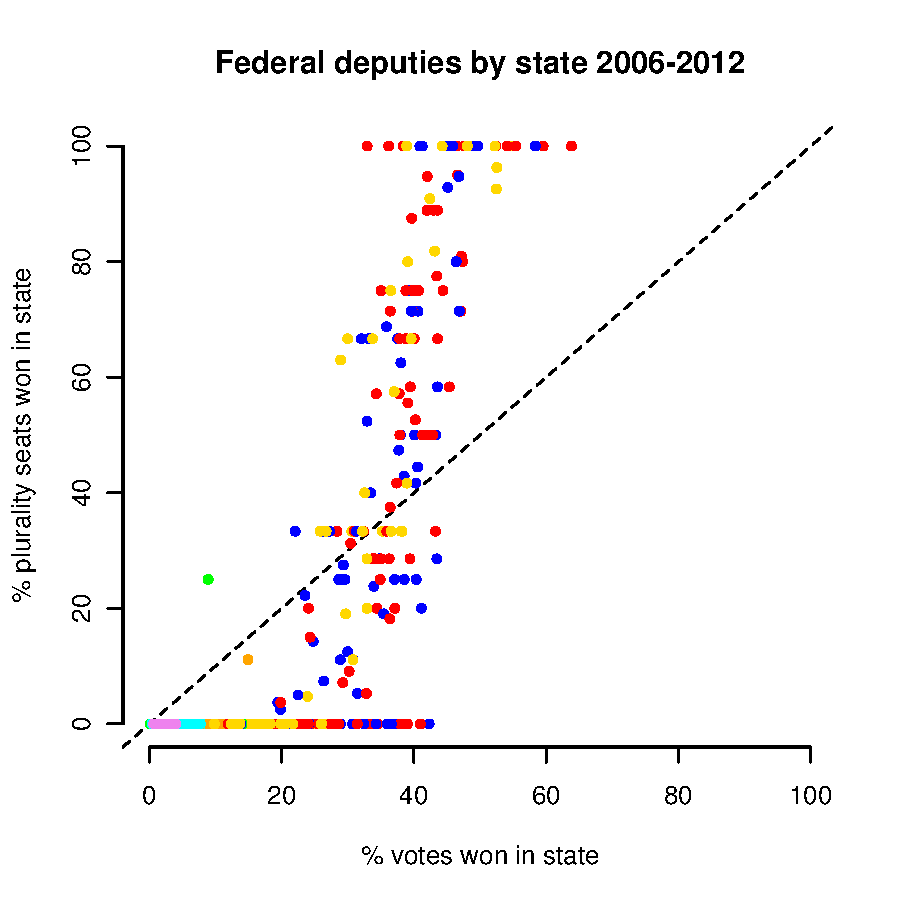
\includegraphics[width=.6\columnwidth]{../graphs/resXedo20062012.pdf} 
\caption{Seats and votes in the states. Each point is a party-state-year, blue for PAN, red for PRI, gold for PRD, other colors for minor parties.}\label{F:seatsVotes}
\end{center}
\end{figure}

\subsection{Two classes of distorsion}

Undue advantage is known, in the specialized literature, as partisan bias, and is one goal that strategic redistricters pursue. It is not, however, alone: scholarship highlights district responsiveness, also know as majoritarian bias, as another goal. These ought to be distinguished \citep[this paragraph draws heavily on][, ch.\ 3]{cox.katz.2002}. Partisan bias helps the beneficiary buy seats with fewer votes than others. Because seat distribution is a constant sum game, bias in favor of someone always implies bias against someone else. One way of introducing party bias in district lines is with the conventional redistricting strategy known as packing: group your adversary's voters in few districts, wasting votes to win unnecessarily safe seats, raising the price of victory. Responsiveness, on the other hand, is the feature granting a seat bonus to large parties. Maximal responsiveness occurs within each single-member district in isolation: the winner takes all, the rest nothing. The same could be achieved in a whole state by drawing lines so that every district is representative of the state's electorate (Cox and Katz's microcosm strategy). The party with most votes wins every seat, maximizing the vote responsiveness of the proposal. 

Formalizing party bias and responsiveness opens the way towards estimation of these district characteristics. The two-party case is simpler and extends to multiparty systems \citep{taagepera.CubeLaw.1973,tufte1973seatsVotes,king.browning1987biasRespUS}. It is a generalization of the cube law stipulating that 

\begin{equation}
 \frac{s}{1-s} = e^\lambda *  \left(\frac{v}{1-v}\right)^\rho \iff
 \texttt{logit}(s) = \lambda + \rho *  \texttt{logit}(v)
\end{equation}\label{E:cubeLaw}

\noindent where $s$ is the seat share that party 1 won with vote share $v$; $\lambda$ is party 1's bias relative to party 2 (positive values favor party 1, negative values favor party 2); and $\rho$ is the districts' responsiveness. With $\lambda=0$ a system with no party bias ensues. Figure \ref{F:lambdaRhoEx} shows how the parameters affect the vote-to-seats conversion. 

\begin{figure}
\begin{center}
    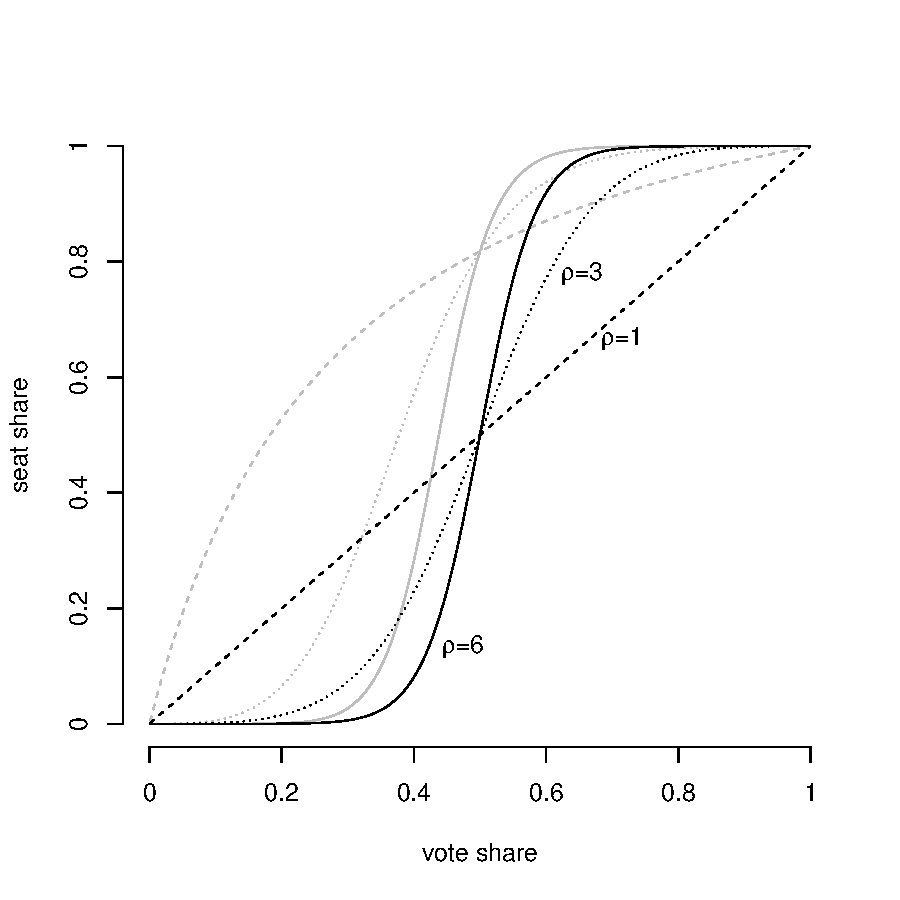
\includegraphics[width=.55\columnwidth]{../graphs/rhoExample.pdf} 
\caption{Illustration of estimated parameters. Party bias is set to $\lambda=0$ in non-grey lines. Grey lines replicate the colored ones with $\lambda=+1.5$.}\label{F:lambdaRhoEx}
\end{center}
\end{figure}

Non-grey lines lack party bias to illustrate variable responsiveness. A system with $\rho=1$ is perfectly proportional representation, the ideal type against which the evaluation of real districts are often contrasted. It appears as the dotted green diagonal: every party winning $x$\% of the vote gets, precisely, $x$\% of seats. $\rho=3$ characterizes the classic cube law, the red curve over-representing the winner (points above the diagonal). Here a party with 55\% of the vote earns two-thirds of the seats, but with 33\% it earns only one-tenth of the seats. As responsivity grows, the curve gets steeper, until barely crossing the majority threshold suffices to win all the available seats. 

Grey lines replicate the values of $\rho$ just discussed but with $\lambda = 1.5$ added. Bias in favor of the party produces a leftward pull of lines. In other words, a bias-favored party requires less effort to reach the threshold for large-party over-representation. (The grey dotted line demonstrates how, due to logit links in Equation 1, party bias also reshapes the function's trace.)

\subsection{Results}

A multiparty and estimable version of equation 1 \citep{king.1990elRespBiasMultiparty} establishes that party $j$'s ($j=1,2,\ldots,J$) expected seat share is 
\begin{equation}
 E(s_j) = \frac{e^{\lambda_j} * v_j^\rho}{\sum_{m=1}^{J} e^{\lambda_m} * v_m^\rho}
\end{equation}

\noindent with data and parameters indexed to identify the parties. \citep[Another, with application to Argentine federalism, is][.]{calvo.micozzi.govReform.2005} Setting $\lambda_2 = 0$, as done below, forces the remainder $\lambda_{j \neq 2}$ to express party bias with relation to the PRI's ($j=2$ for this party in the dataset). This is convenient to test the presumption of PRI-favoring bias:. if present, $\hat{\lambda}_{j \neq 2}<0$ would result.

A common estimation strategy relies on a time-series of national aggregates. This is what M\'arquez has done for eight elections 1991--2012, uncovering substantive anti-PAN bias and high responsiveness. The estimation strategy here, as before, is with state-level data. One disadvantage of the approach is that states have few districts (9.4 on average), and this will amplify the system's responsiveness \citep{taagepera.CubeLaw.1973}. But the advantages are many, like mutiplying observations. This is evident in Figure \ref{F:seatsVotes}, with many points despite reporting three elections only. It also holds the actual district structure constant --- redistricting in 1996 and 2004--05 invalidate district comparability before and after. And it takes advantage in the variation of state party systems (this report fails to take full advantage of this variance, but this could be exploited for the APSA paper). 

\begin{figure}
\begin{center}
  \begin{tabular}{cc}
    (a) & (b) \\
    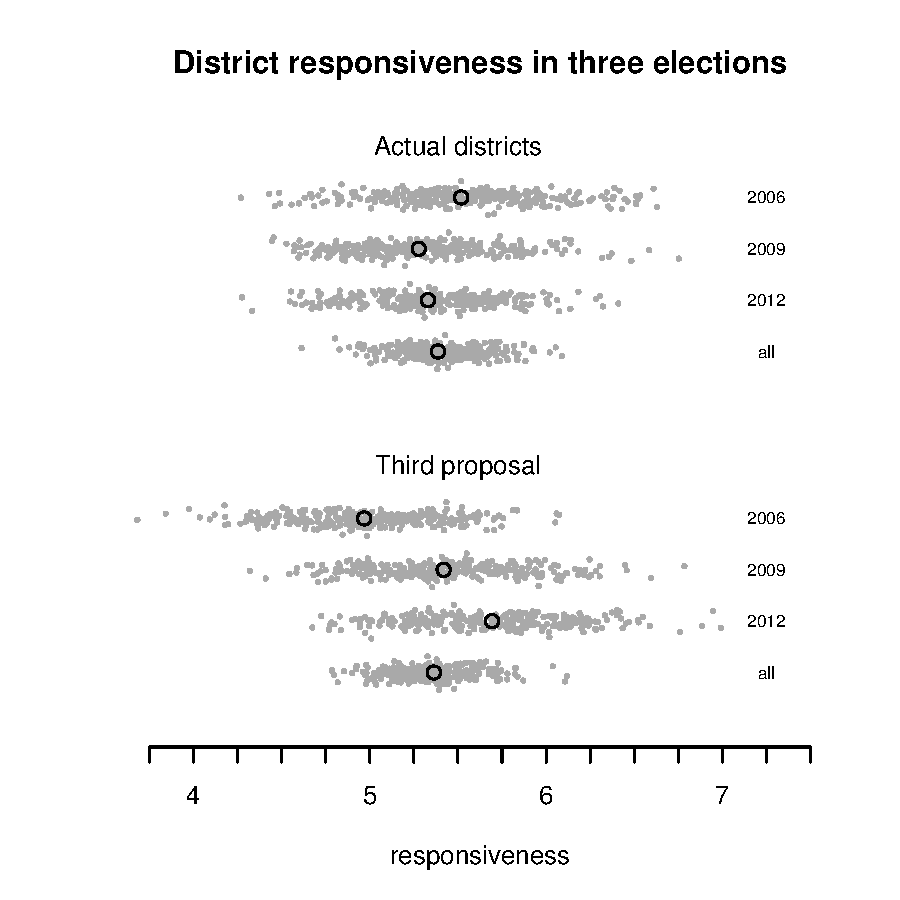
\includegraphics[width=.45\columnwidth]{../graphs/resp200612s0s3.pdf} &
    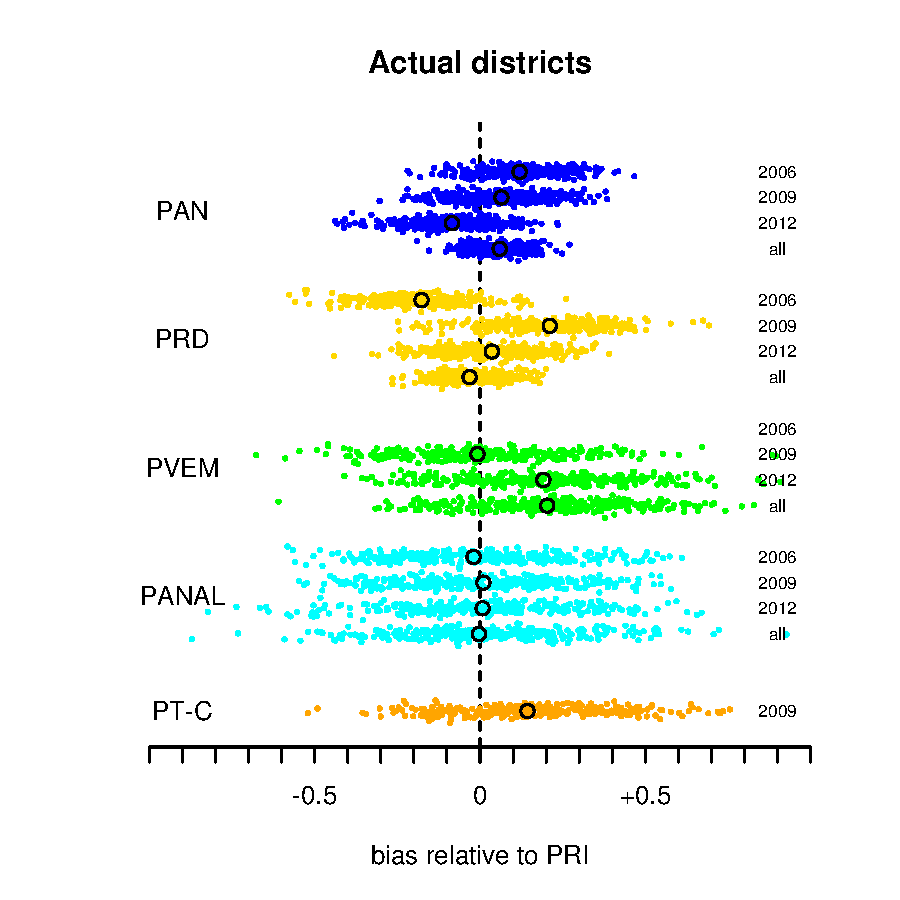
\includegraphics[width=.45\columnwidth]{../graphs/bias200612s0.pdf} \\
    (c) & (d) \\
    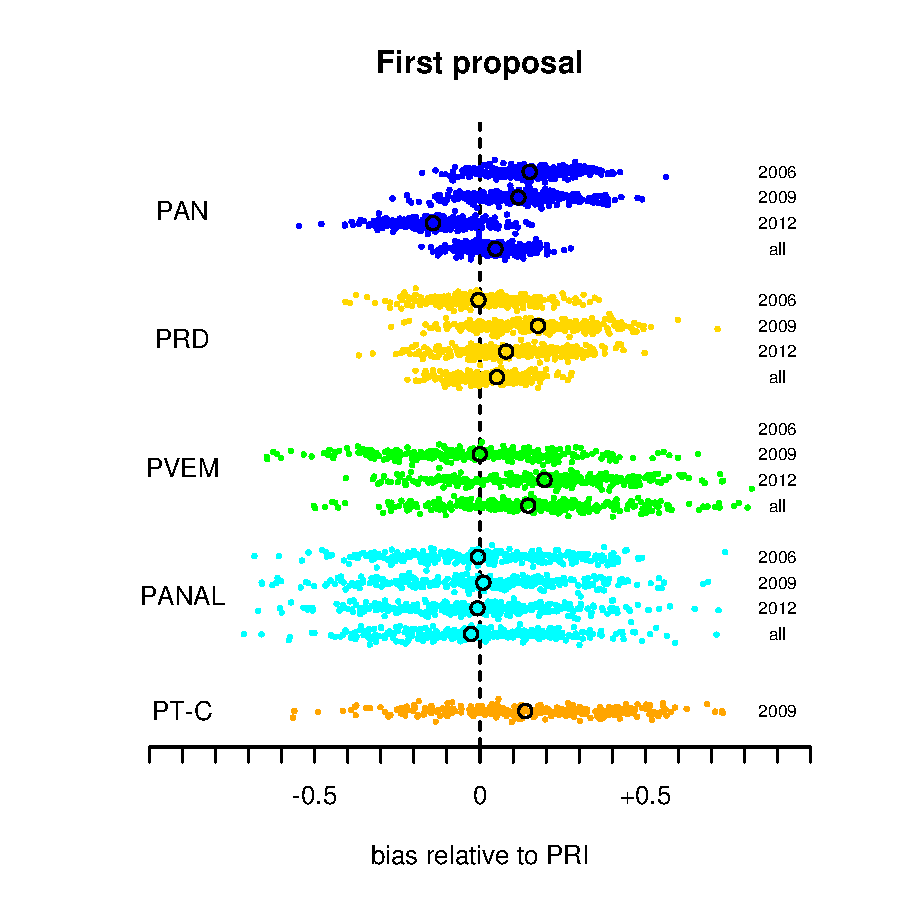
\includegraphics[width=.45\columnwidth]{../graphs/bias200612s1.pdf} &
    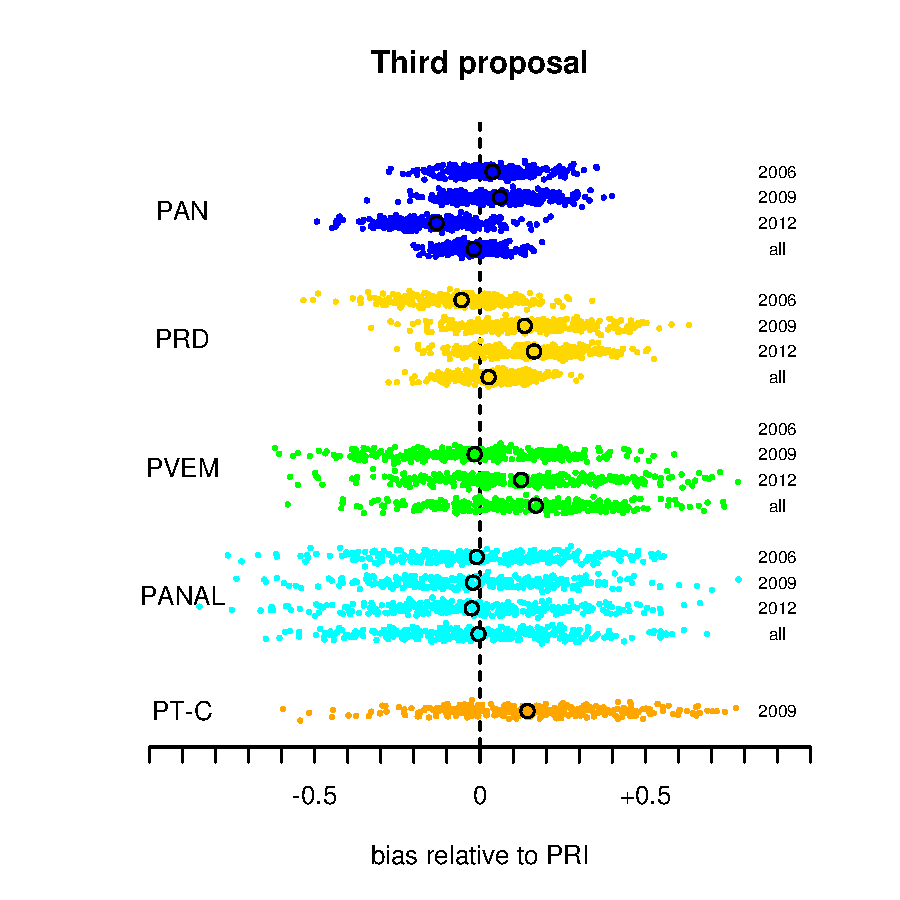
\includegraphics[width=.45\columnwidth]{../graphs/bias200612s3.pdf} 
  \end{tabular}
  \caption{Redistricting, responsiveness, and party bias. Plots report the posterior sample of model's parameters $\lambda_j$ for four parties and $\rho$, and the median value (black circles).}\label{F:posterior_s0s1s3}
\end{center}
\end{figure}


The  method of estimation is MCMC \citep{jackman.2000}.\footnote{Three chains were iterated 10 thousand times, taking every fiftieth observation of the last 5 thousand to sample the posterior distribution. Convergence was gauged visually with traceplots of the separate chains for each of the model's parameters. Estimation performed with JAGS \citep{jags.cite}, implemented from R \citep{r.cite} using package R2jags \citep{r.r2jags}. Data and code to replicate the analysis can be found at HTTP.} As expected, district responsiveness is extremely high, between 5 and 6 depending on the year selected (the steepest line in illustrative Figure \ref{F:lambdaRhoEx} has $\lambda=6$). Figure \ref{F:posterior_s0s1s3}.a reports point estimates (the black circles are the median of the posterior sample of the responsiveness parameter) for each year separately, all years pooled together, and comparing actual districts to the first and third redistricting proposals. Estimate precision is assessed with the cloud of grey points (technically, it is the full sample of posterior $\rho$s). The redistricting proposal makes little change to district responsiveness, it just makes it slightly more volatile from one election to next. Owing to few districts per state, the estimated responsiveness at the state level ($\hat{\rho} \approx 5.5$) is twice M\'arquez's nationwide ($\hat{\rho} = 2.6$). All three parties experience situations of large party bonus and small party penalty that, to a good extent, cancel each other in the national statistic.

Regarding party bias, signals that are not weak all tend to be accompanied by a good deal of noise, with few exceptions. At the national level, and over a longer haul, M\'arquez discovers bias in favor of the PRI, but mostly in favor of the PRD, and against the PAN, that seems not the product of chance alone. Analysis at the state-level reveals no such biases. As said, Figures \ref{F:posterior_s0s1s3}.b--d express bias relative to the PRI. Although PAN experienced weak signal in its favor in the whole 2006--12 period, a fair density of the blue cloud is, in fact, negative. PRD vs.\ PRI bias is clearly centered at zero in the full period. The left did experience significant bias in isolated years: against in 2006, in favor in 2009. Perhaps voters who strategically abandoned the hopeless PRI presidential candidate in 2006 to vote for L\'opez Obrador did not also endorse the PRD's congressional candidates. No other year for no other party reveals any bias unaccompanied by much noise.

Comparing the proposals and the status quo shows that the redistricting proposals make a difference in few cases. The PAN in 2012 is noe, suffering negative bias compared to the PRI that mostly exceeds noise. The PRD bias signals for 2006 and 2009 under the status quo become milder under both proposals.   

\section{State's representation in Congress}

Redistricting begins with a process to apportion seats in the chamber of deputies for every state according to its population, as in the U.S. This has been done with the Hamilton method of largest remainders,\footnote{The quota $Q$ (or price) of a seat is the country's population divided by the number of seats in the chamber (300 since 1979). A first allocation is made to each state by dividing its population by $Q$, rounded down. Unallocated seats, if any, are awarded to states with largest fractional remainders. See \citet{balinskiYoung2001FairRep}.} with little if any debate about alternative methods. 

Two patterns are noteworthy. Redistricting has reduced largest distorsions without wiping them nor attempting to prevent foreseeable distorsion due to rapid demographic change. DF retained a one deputy over-representation (down from >7) in 1997, and +2 in 2005. Meanwhile Mexico State remained at $-5$ in 1996, at $-1$ in 2004.   

\begin{figure}
\begin{center}
  \begin{tabular}{cc}
    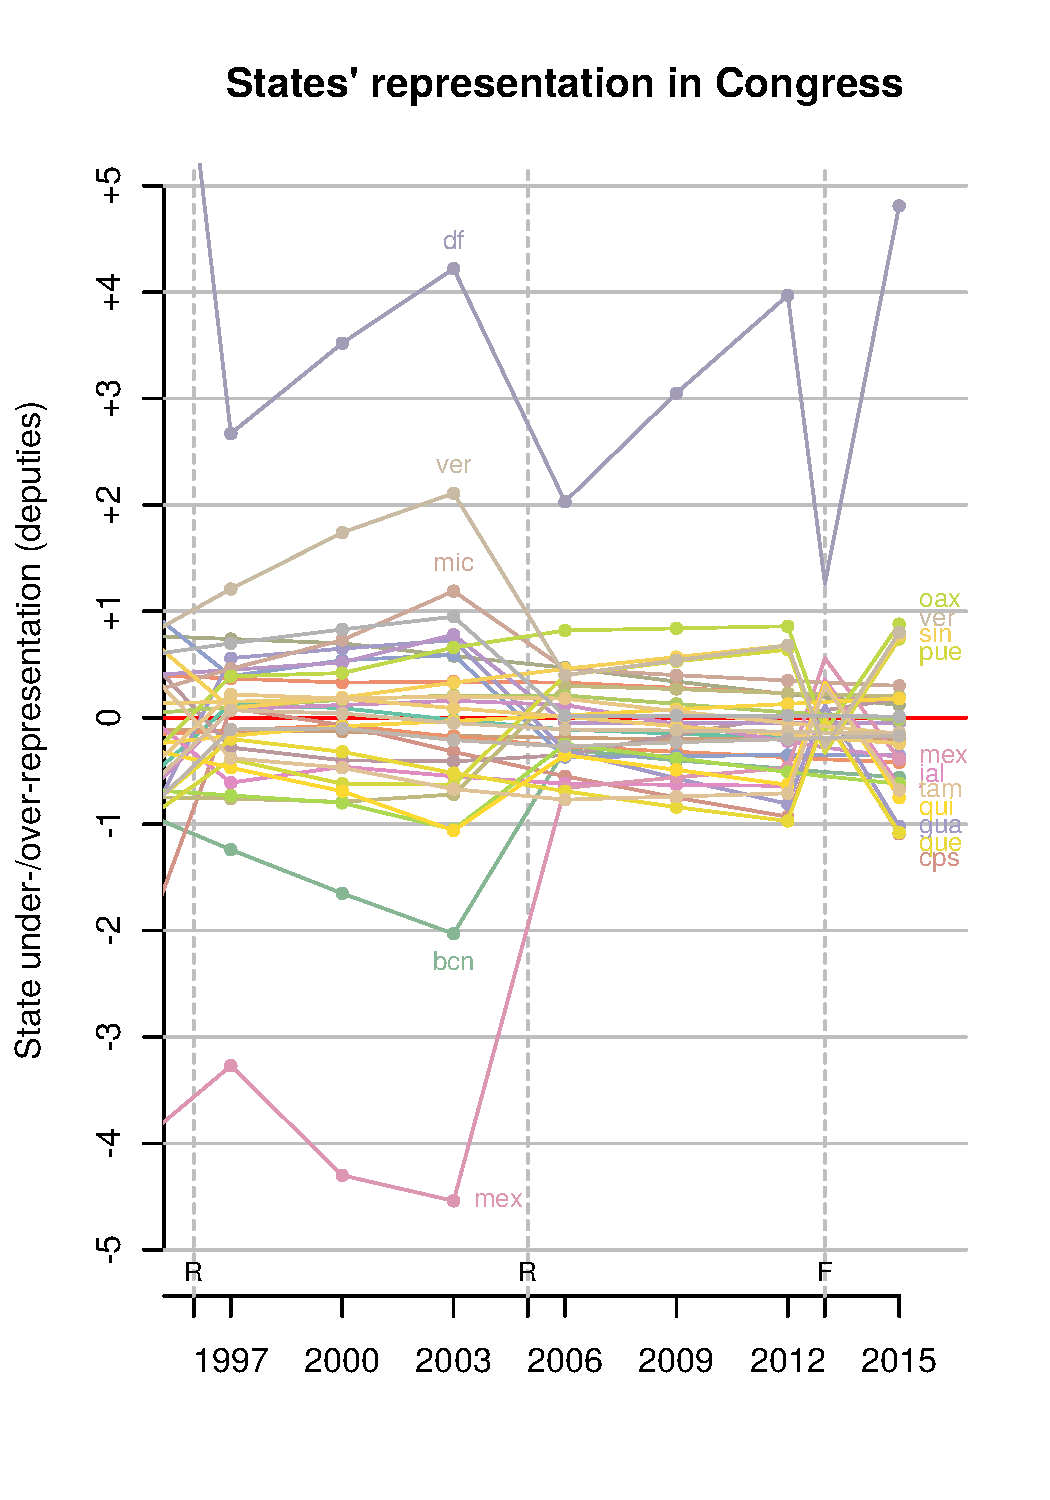
\includegraphics[width=.5\columnwidth]{../graphs/statesUnderOverRep.pdf} & 
    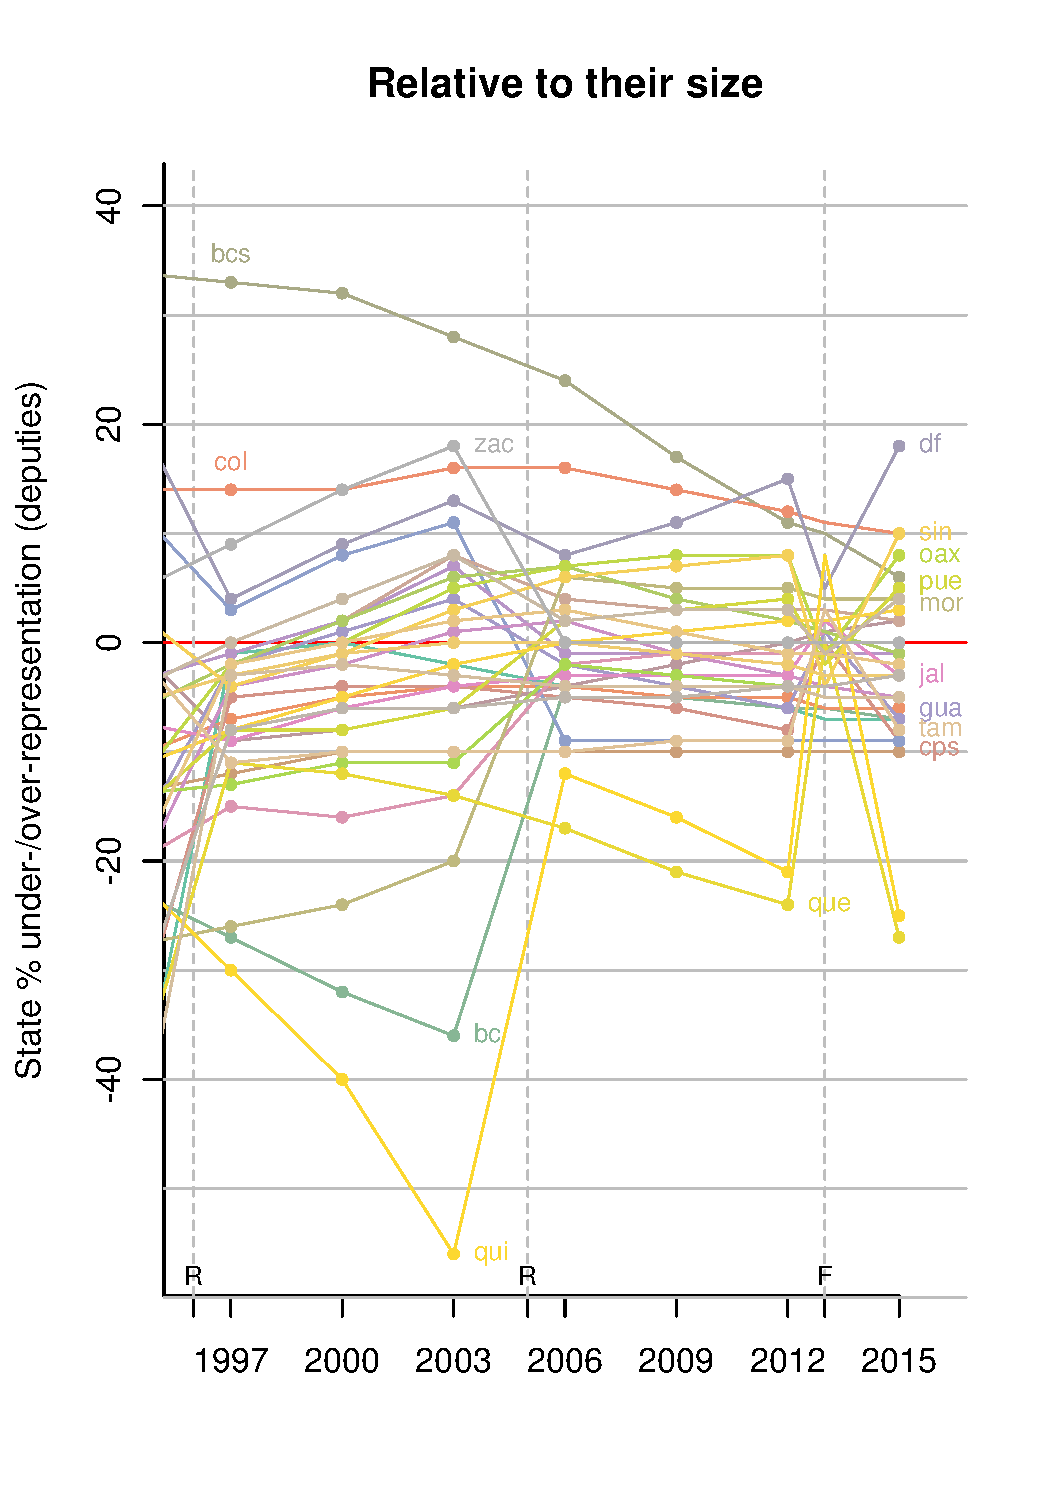
\includegraphics[width=.5\columnwidth]{../graphs/statesUnderOverRep-rel.pdf} \\ 
  \end{tabular}
  \caption{Demography and state apportionment. Lines connect the lower chamber seats aportioned to seats due difference for each state over time. Letters R in the horizontal axis indicate redistricting, letter F a failed redistricting attempt (reporting the effect it would have had).}\label{F:underOverRep}
\end{center}
\end{figure}

\begin{tabular}{l|c|c|}
State          & \mc{2}{c}{Would 2013 have reverted?}\\ \cline{2-3}
representation & yes                  & no \\ \hline
               &                      & cua gue hgo mic mor  \\ 
On target      & jal mex ver          & nay nl san son tab  \\ 
               &                      & tla yuc zac \\ \hline
Over           & df oax pue sin       & bcs col\\ \hline
Under          &  cps gua que qui tam & ags bc cam coa dgo\\ \hline
\end{tabular}


\section{District similarity after redistricting}

The similarity index \citep[][:15--7]{cox.katz.2002} captures how much districts change with the redistricting process. The method identifies the parent district or single largest contributor of population to every new district. The similarity index $s$ divides the population that parent and new district share in common ($c$) by their joint population: $s = c / (p + n - c)$. Its range is zero (if they share no population at all) to one (if districts are identical). 

\begin{tabular}{lrrrrr}
redistricting &        &        &        &       &      \\
proposal      &   min  &  25\%  & median &  75\% &  max \\ \hline
first         & 0.125  & 0.437  & 0.643  & 0.805 &  1   \\
third         & 0.128  & 0.419  & 0.584  & 0.755 &  1   \\
\end{tabular}


\section{Malapportionment}

\begin{figure}
\begin{center}
  \begin{tabular}{cc}
    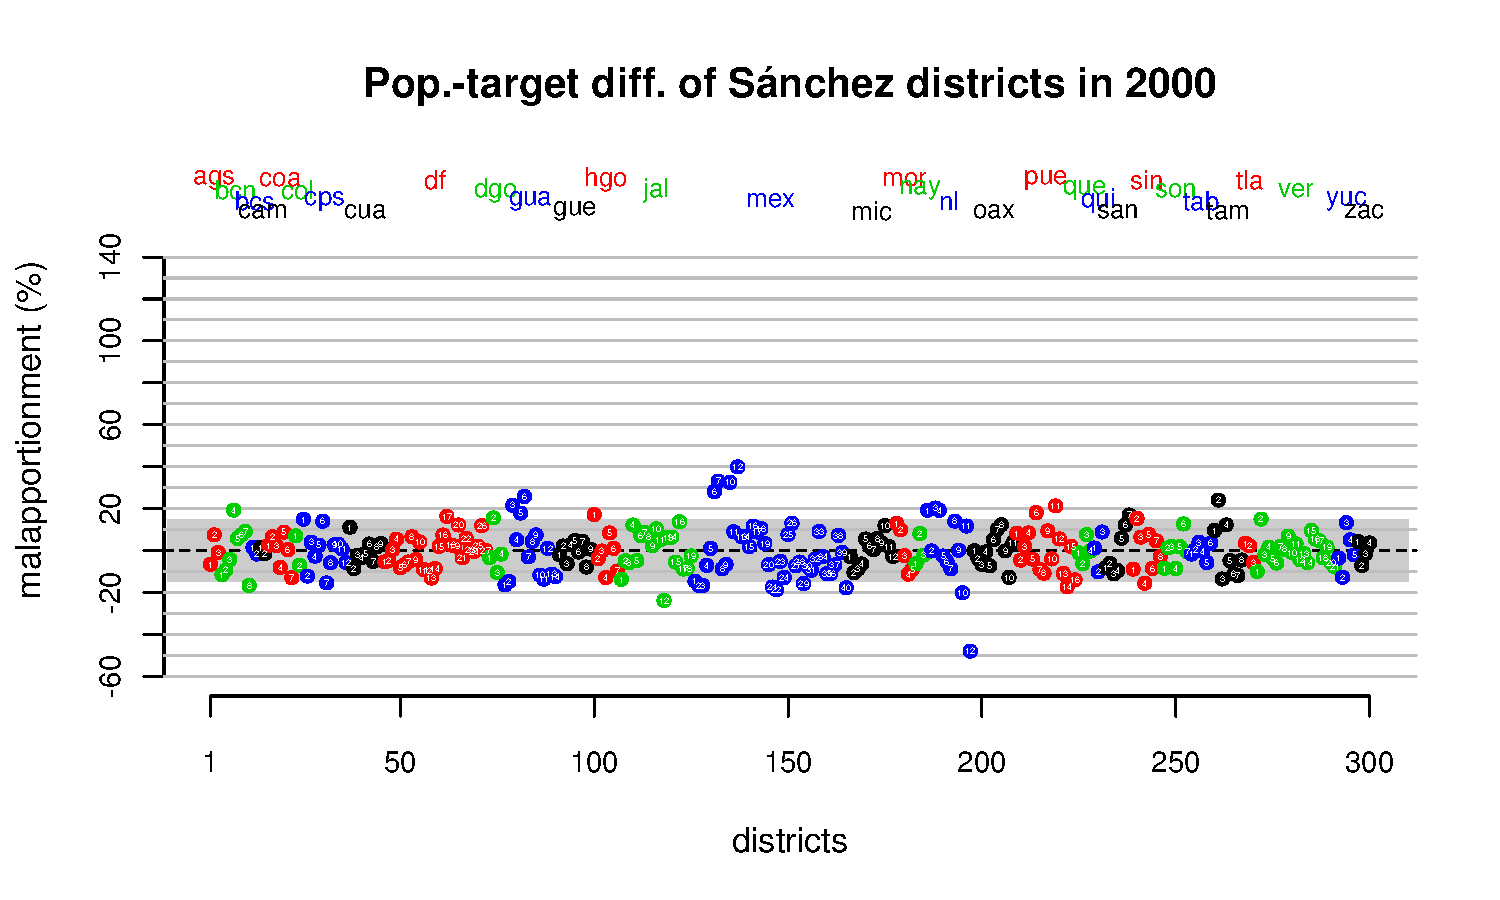
\includegraphics[width=.5\columnwidth]{../graphs/malapp2000d0.pdf} & \\
    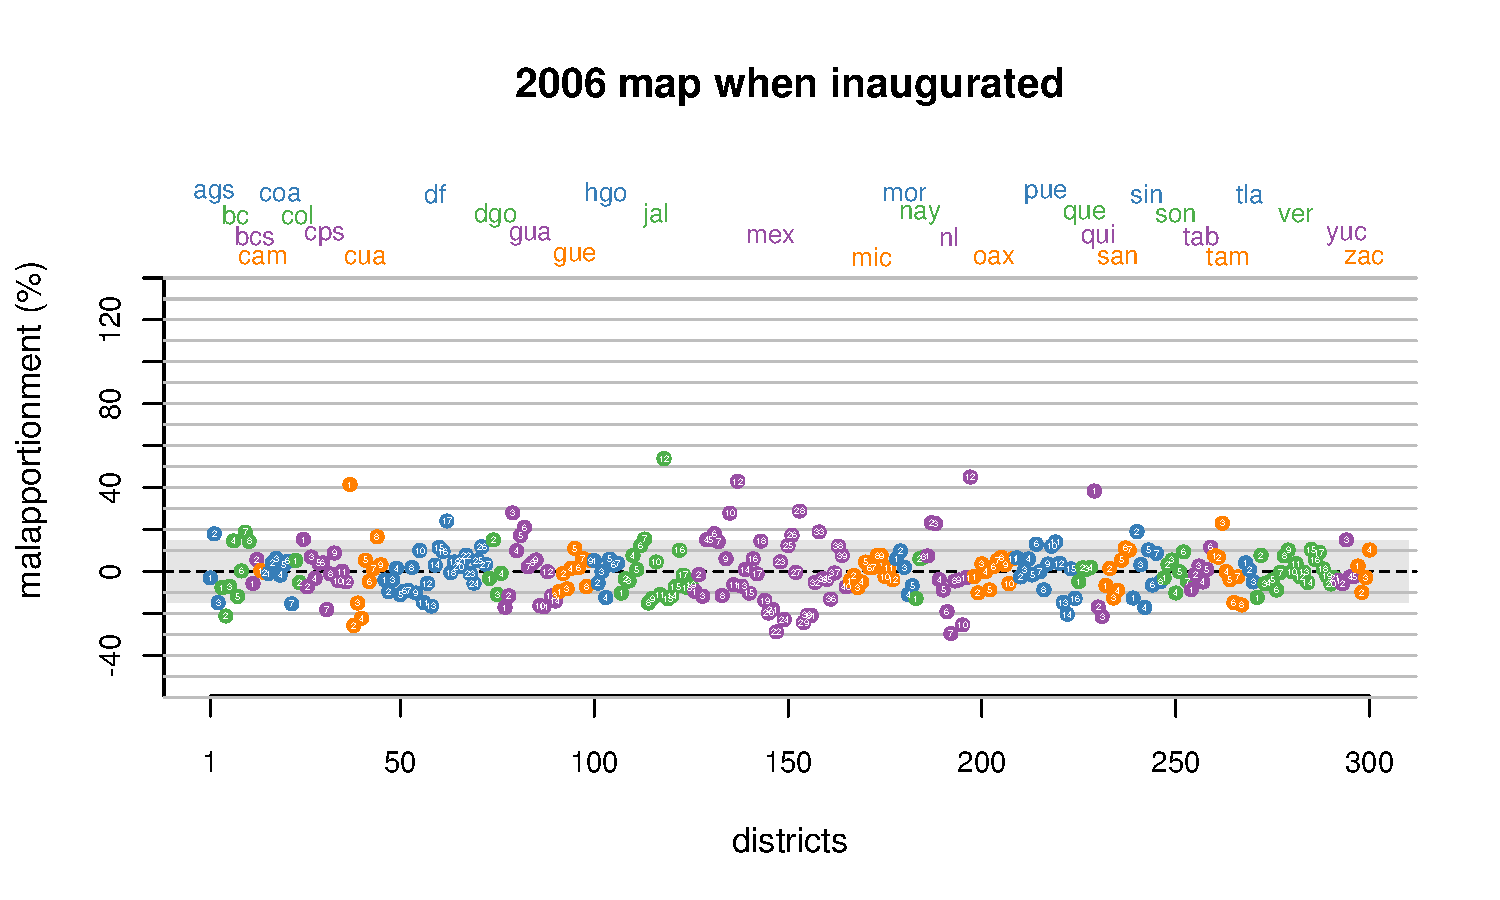
\includegraphics[width=.5\columnwidth]{../graphs/malapp2006d0.pdf} & \\
    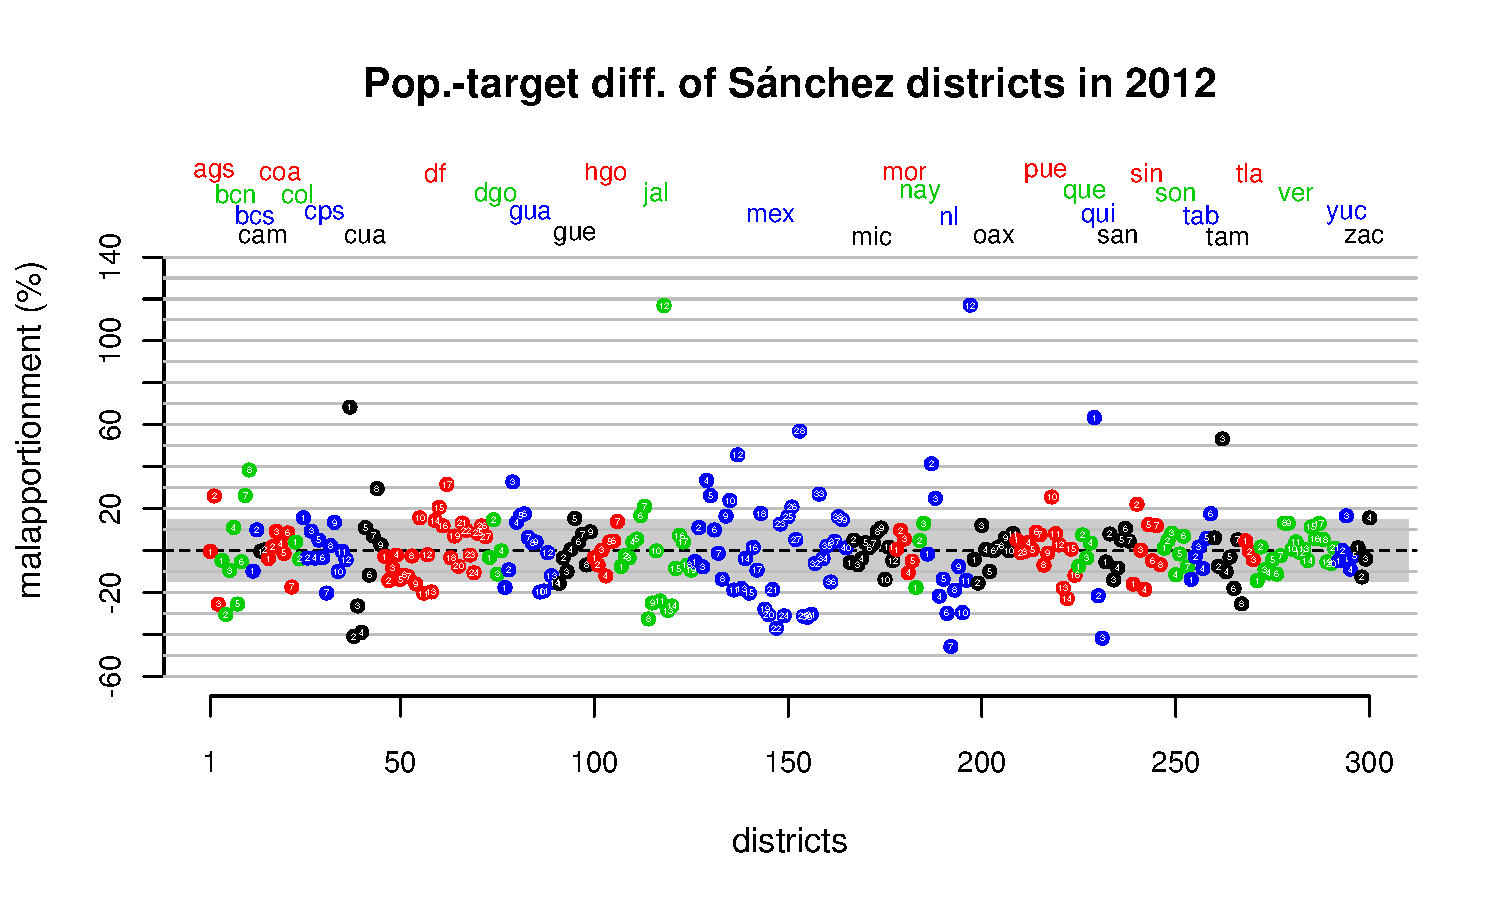
\includegraphics[width=.5\columnwidth]{../graphs/malapp2012d0.pdf} & 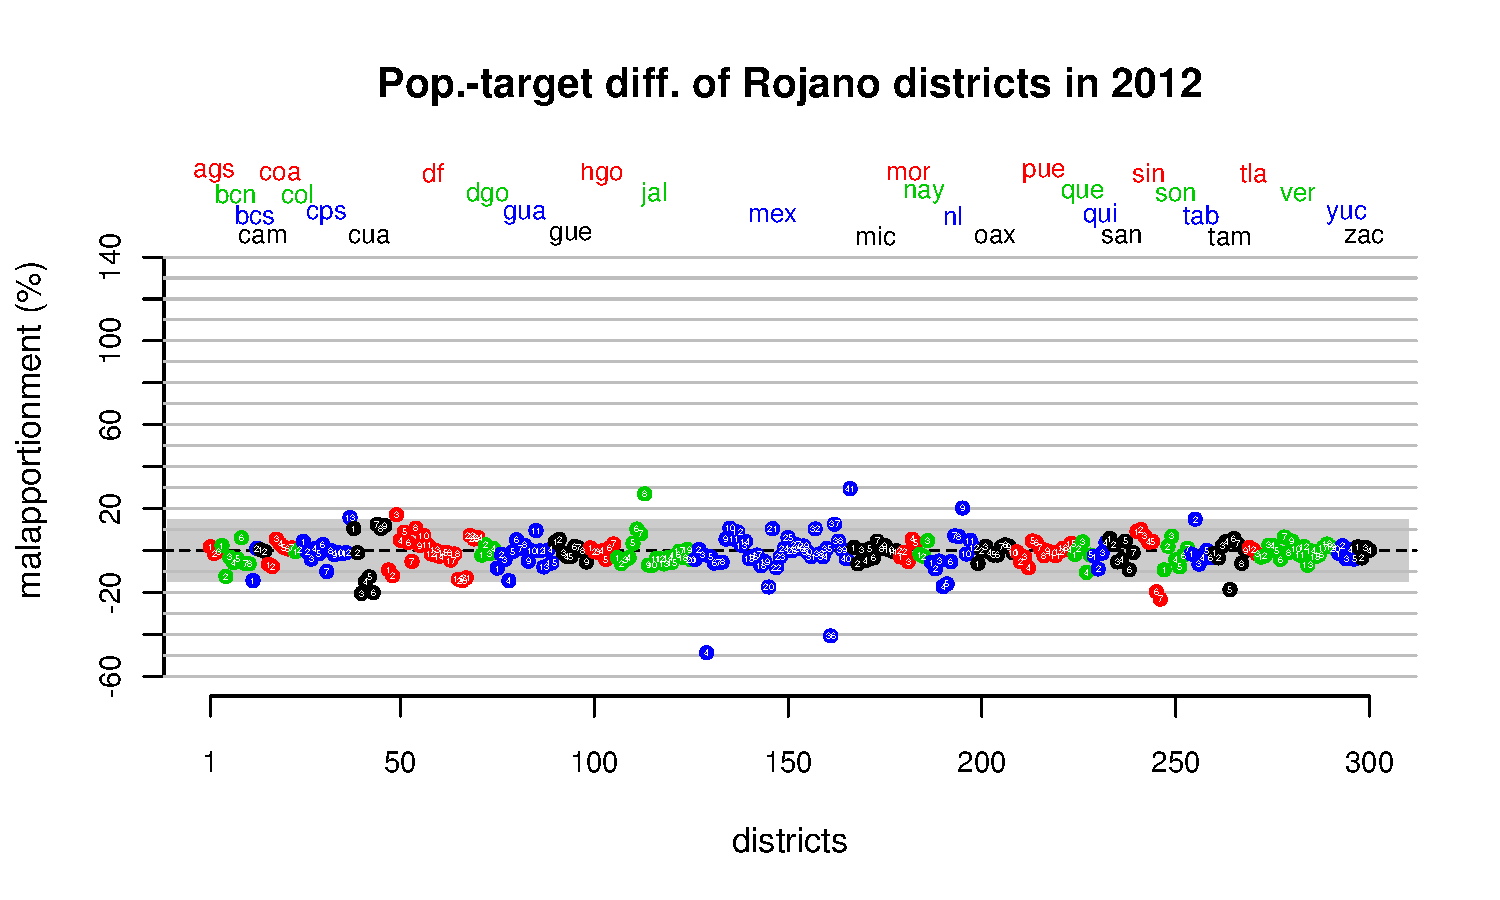
\includegraphics[width=.5\columnwidth]{../graphs/malapp2012d3.pdf} \\
    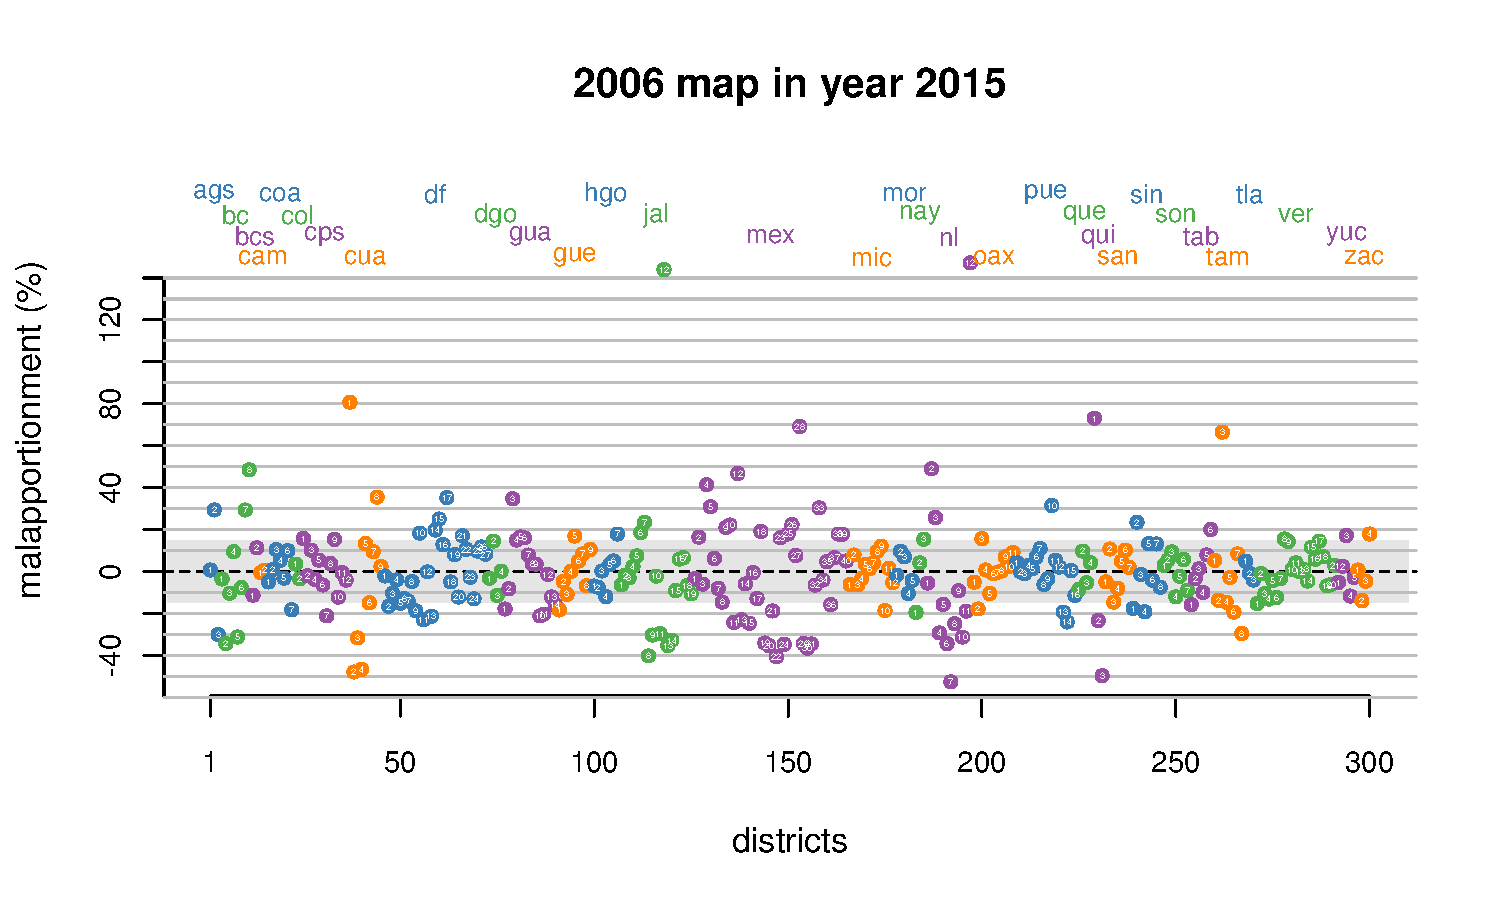
\includegraphics[width=.5\columnwidth]{../graphs/malapp2015d0.pdf} & 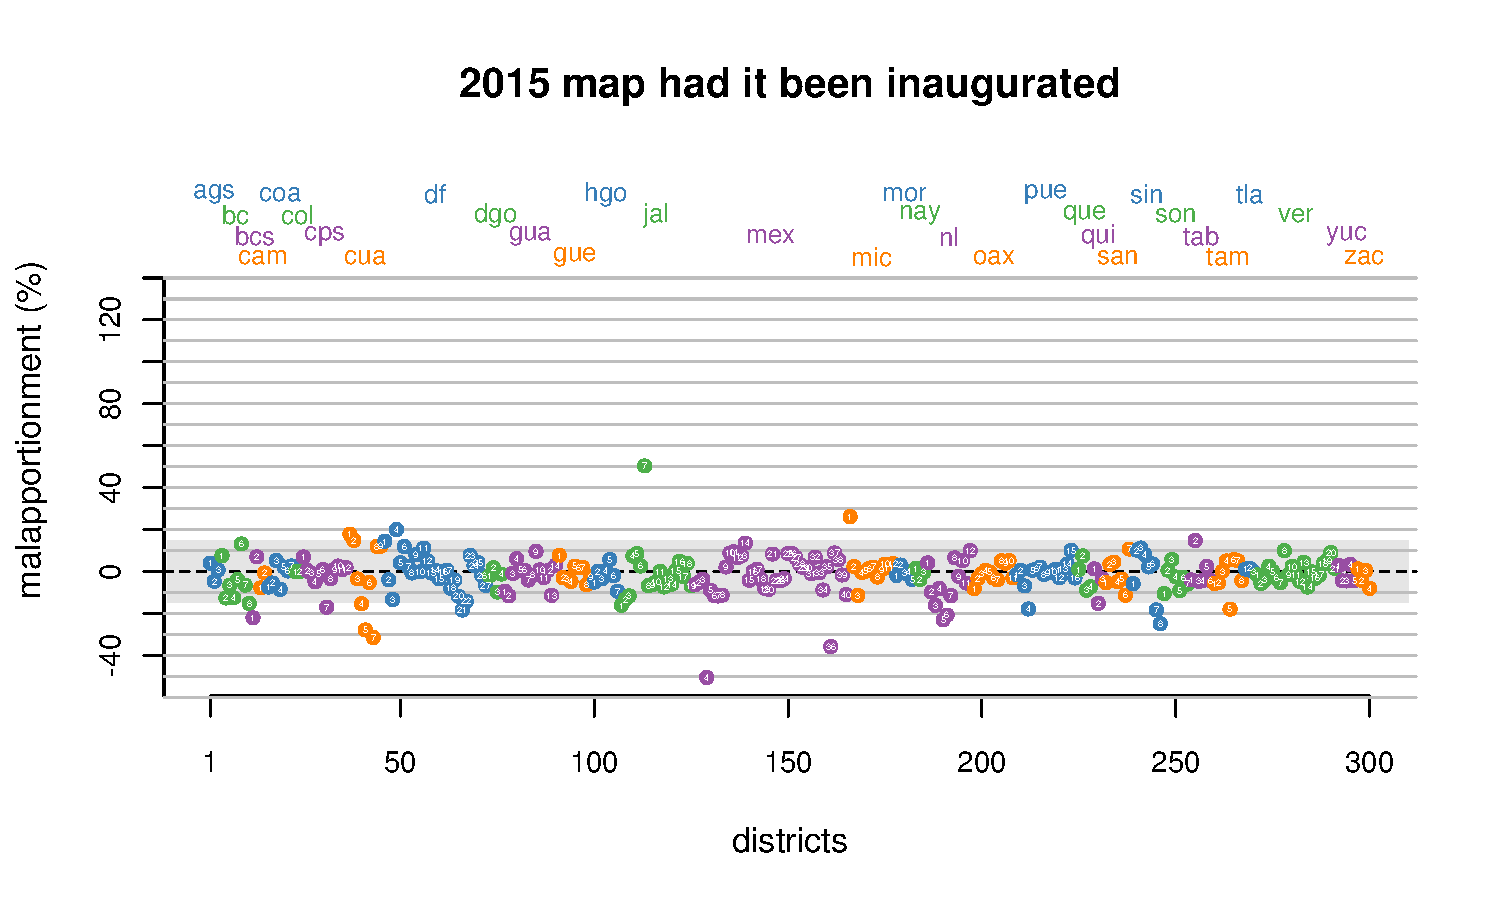
\includegraphics[width=.5\columnwidth]{../graphs/malapp2015d3.pdf} \\
  \end{tabular}
  \caption{Malapportionment through the years}\label{F:malapp}
\end{center}
\end{figure}

IFE is remarkably tolerant to malapportionment. Fifteen percent of over- or under-population in the districts it prepared was considered normal in 1996 and 2013, with no attempt to tend towards zero malapportionment. In 2005 that threshold was 10 percent. Figure \ref{F:malapp} shows how the tolerance band is uniformly occupied by districts even right after inception. I use 2005 partial census and 2010 census to estimate population. IFE began redistricting before the 2005 data existed, using the 1995--2000 period to infer population growth. My linear estimate uses data around estimation points (interpolate, not extrapolate, which should be more precise). The year 2000 plot in Figure \ref{F:malapp} is in fact an extrapolation of that year's population with my method. 

[Get 2000 census at section level to have a better proxy (2000--2005) of IFE's population estimates... source of error]


\begin{tabular}{rcc}
     & \mc{2}{c}{Mean absolute malapportionment} \\
Year & S\'anchez districts & Rojano districts \\
2000 &       7.8           &                  \\  
2006 &       8.9           &                  \\  
2012 &      12.5           &     4.9          \\  
2015 &      14.3           &     6.3          \\  
\end{tabular}

\section{Malapportionment and margin}

\begin{figure}
\begin{center}
  \begin{tabular}{cc}
    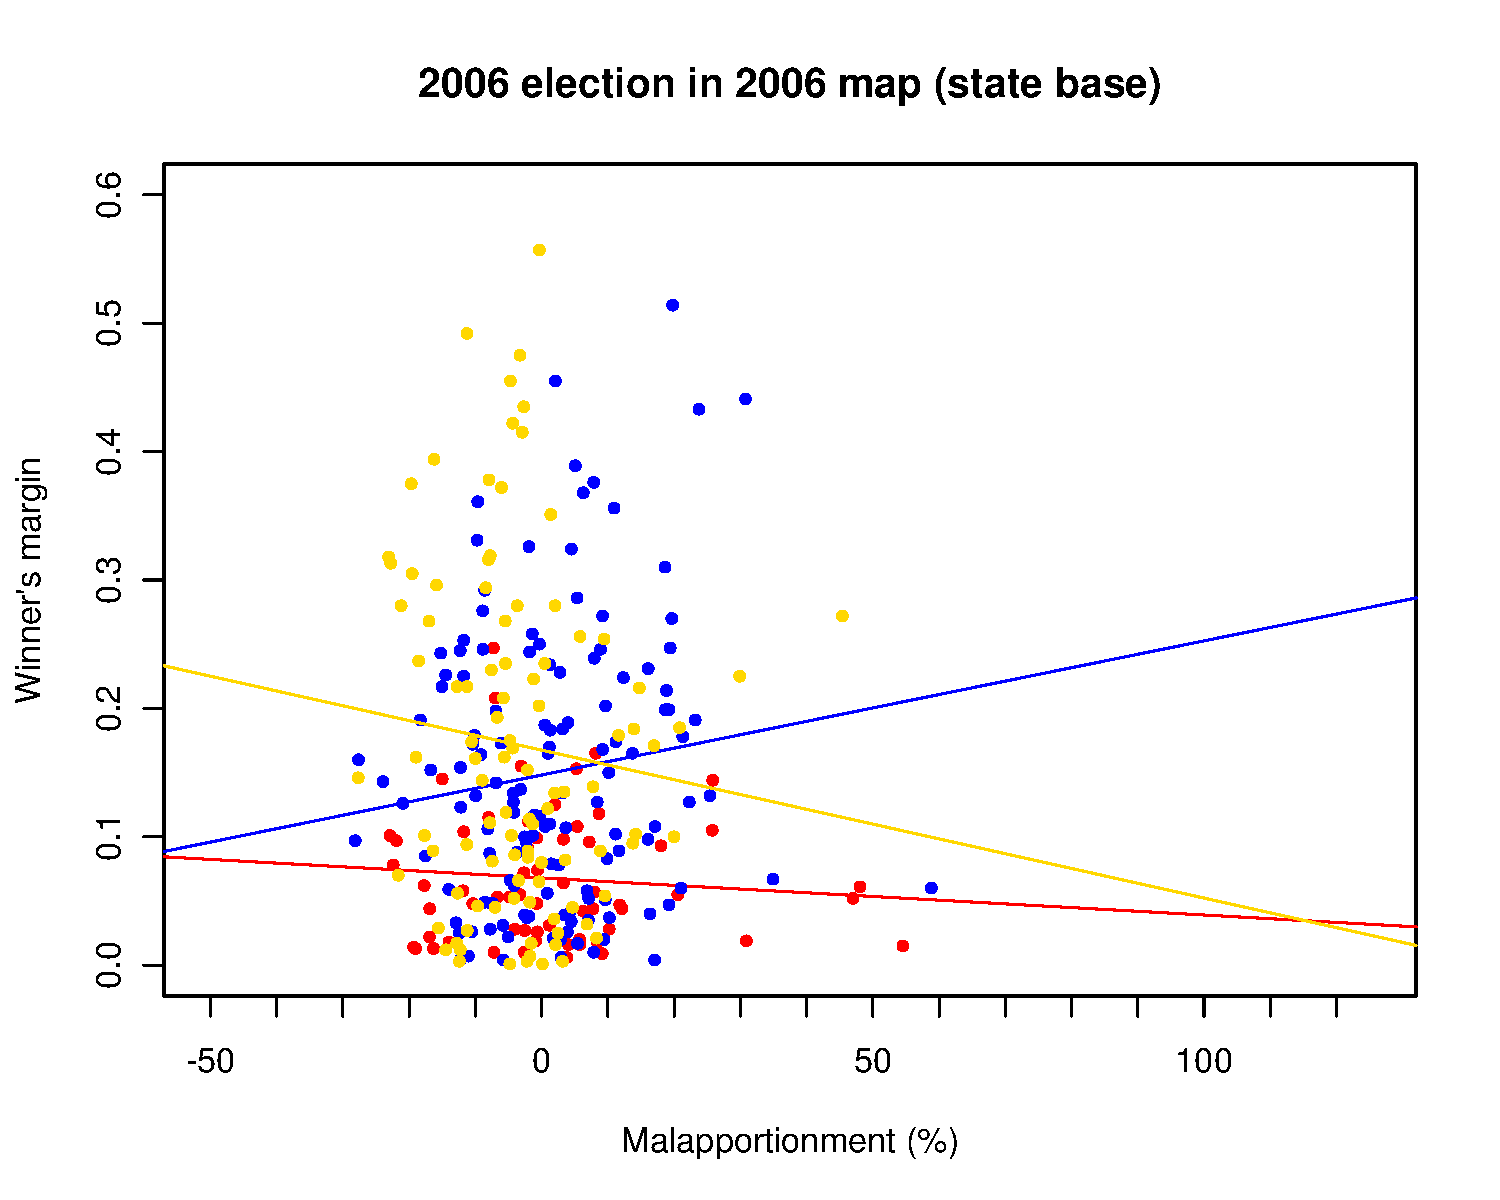
\includegraphics[width=.4\columnwidth]{../graphs/malmg2006d0nat.pdf} & 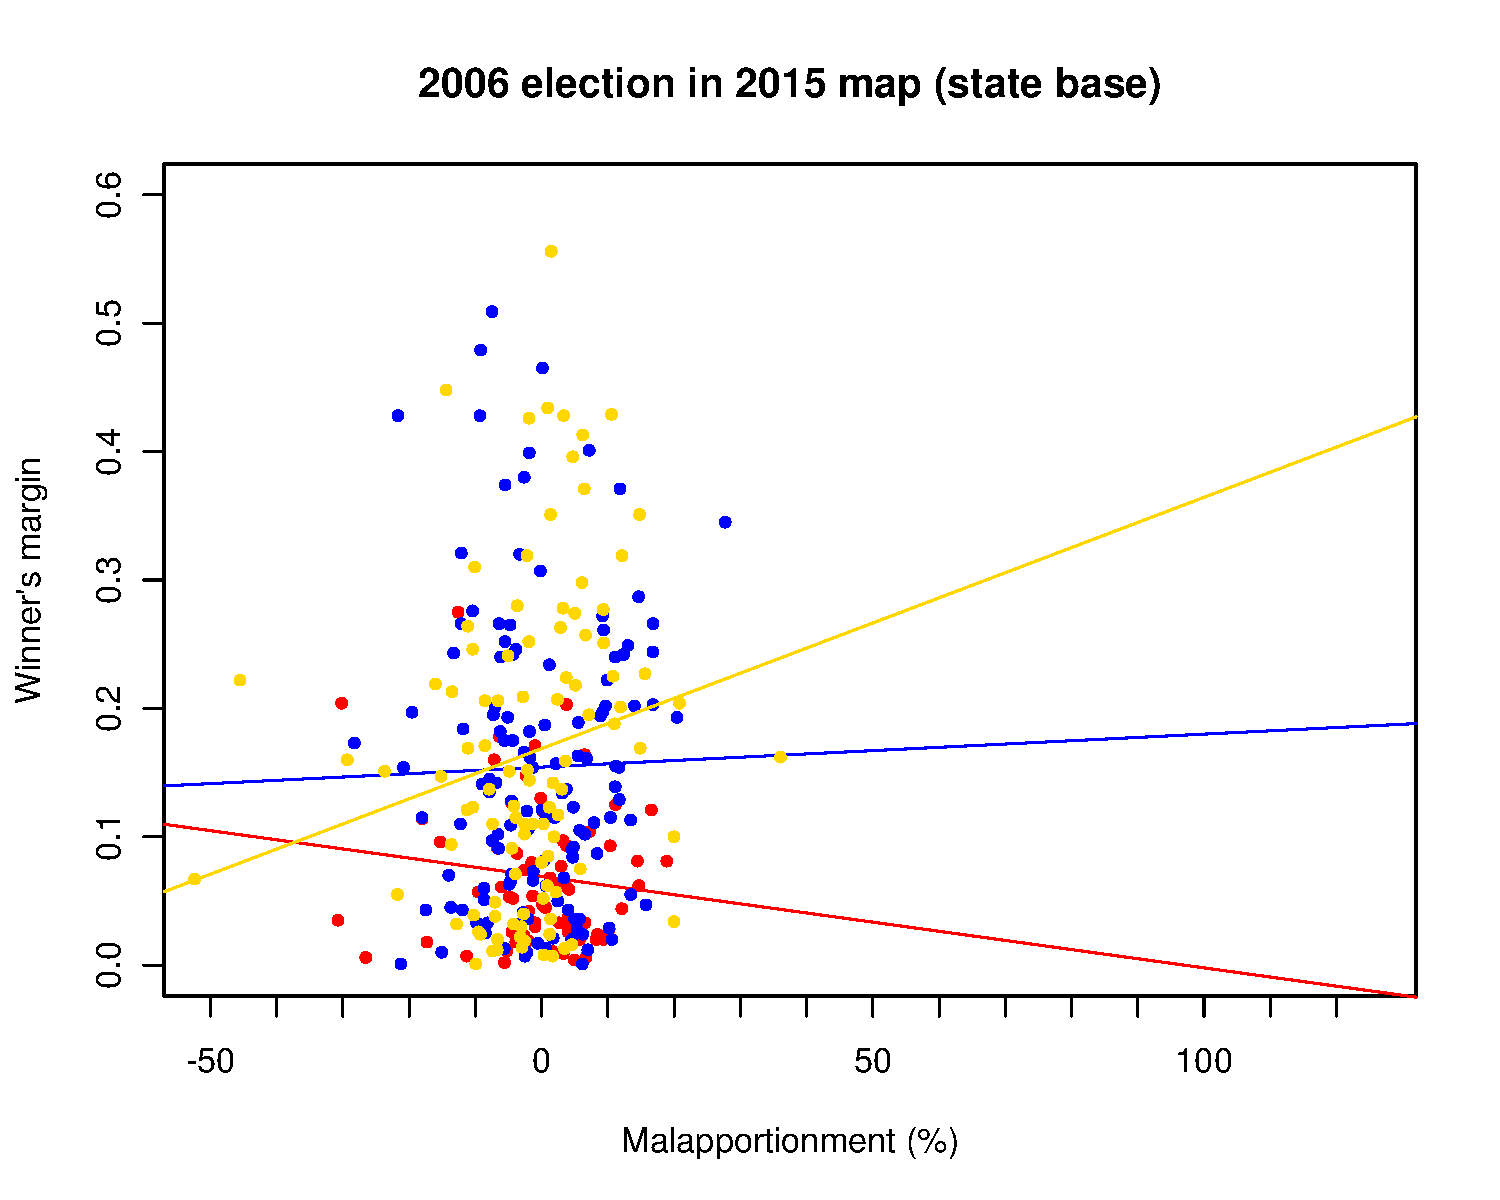
\includegraphics[width=.4\columnwidth]{../graphs/malmg2006d3nat.pdf} \\
    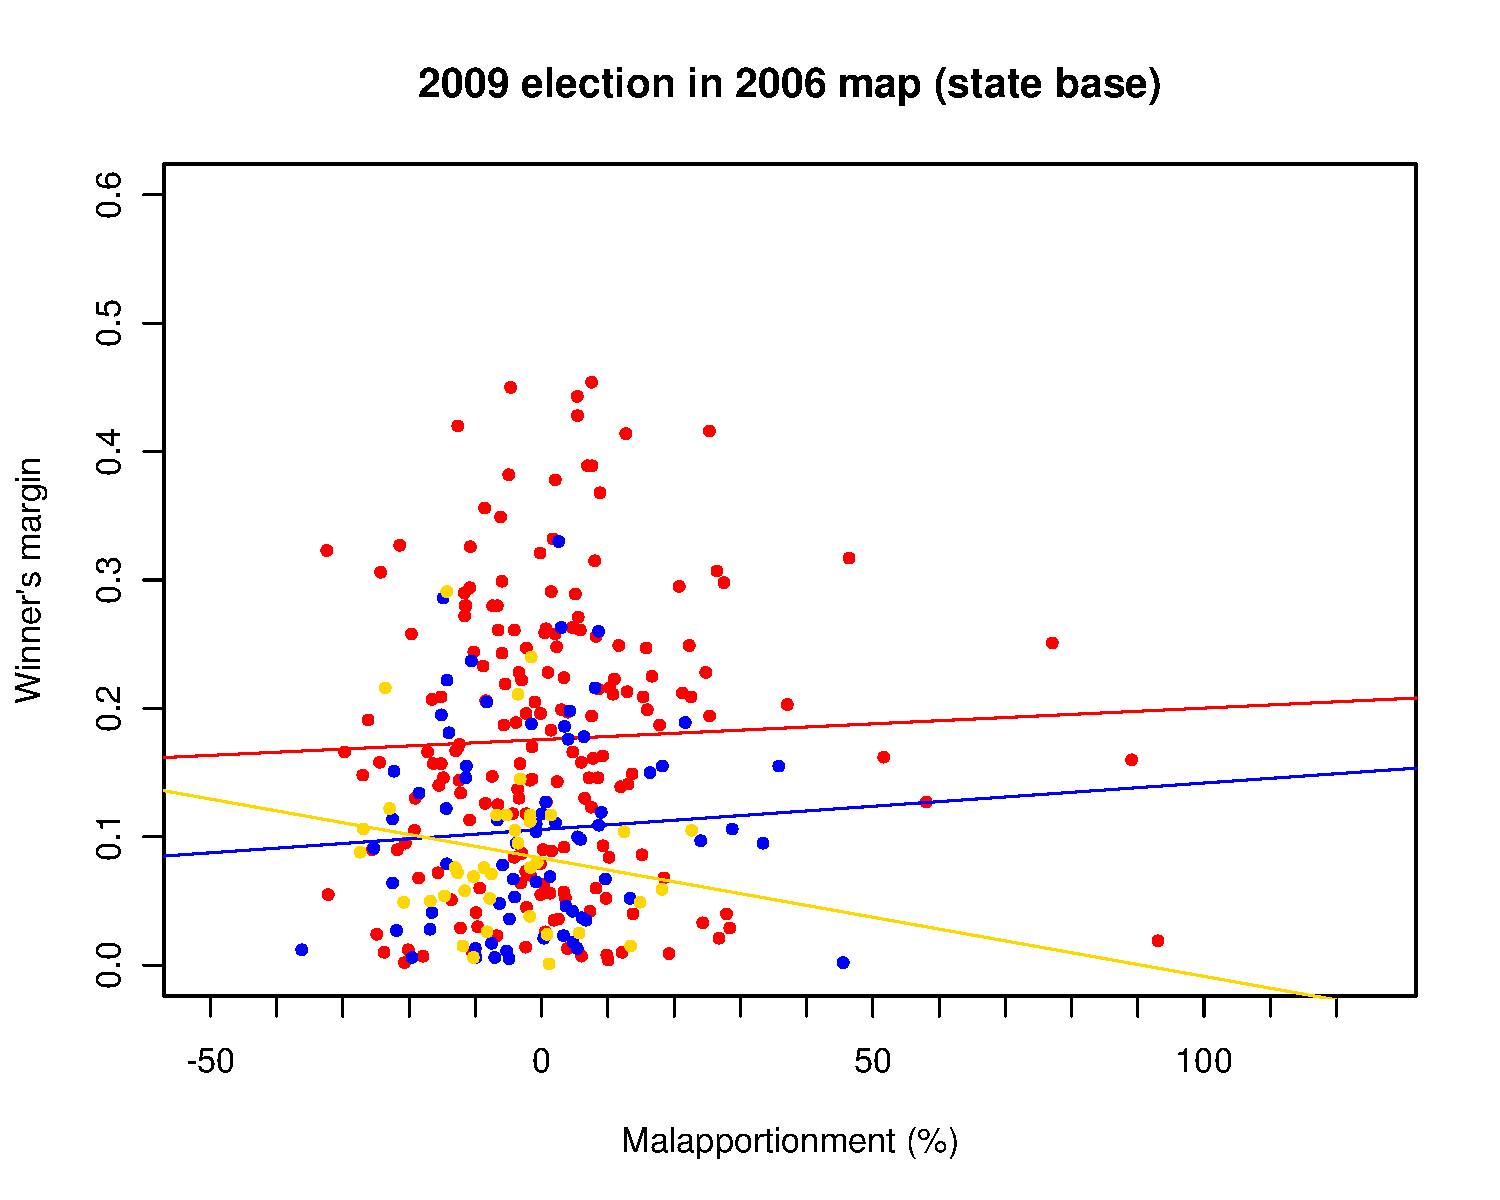
\includegraphics[width=.4\columnwidth]{../graphs/malmg2009d0nat.pdf} & 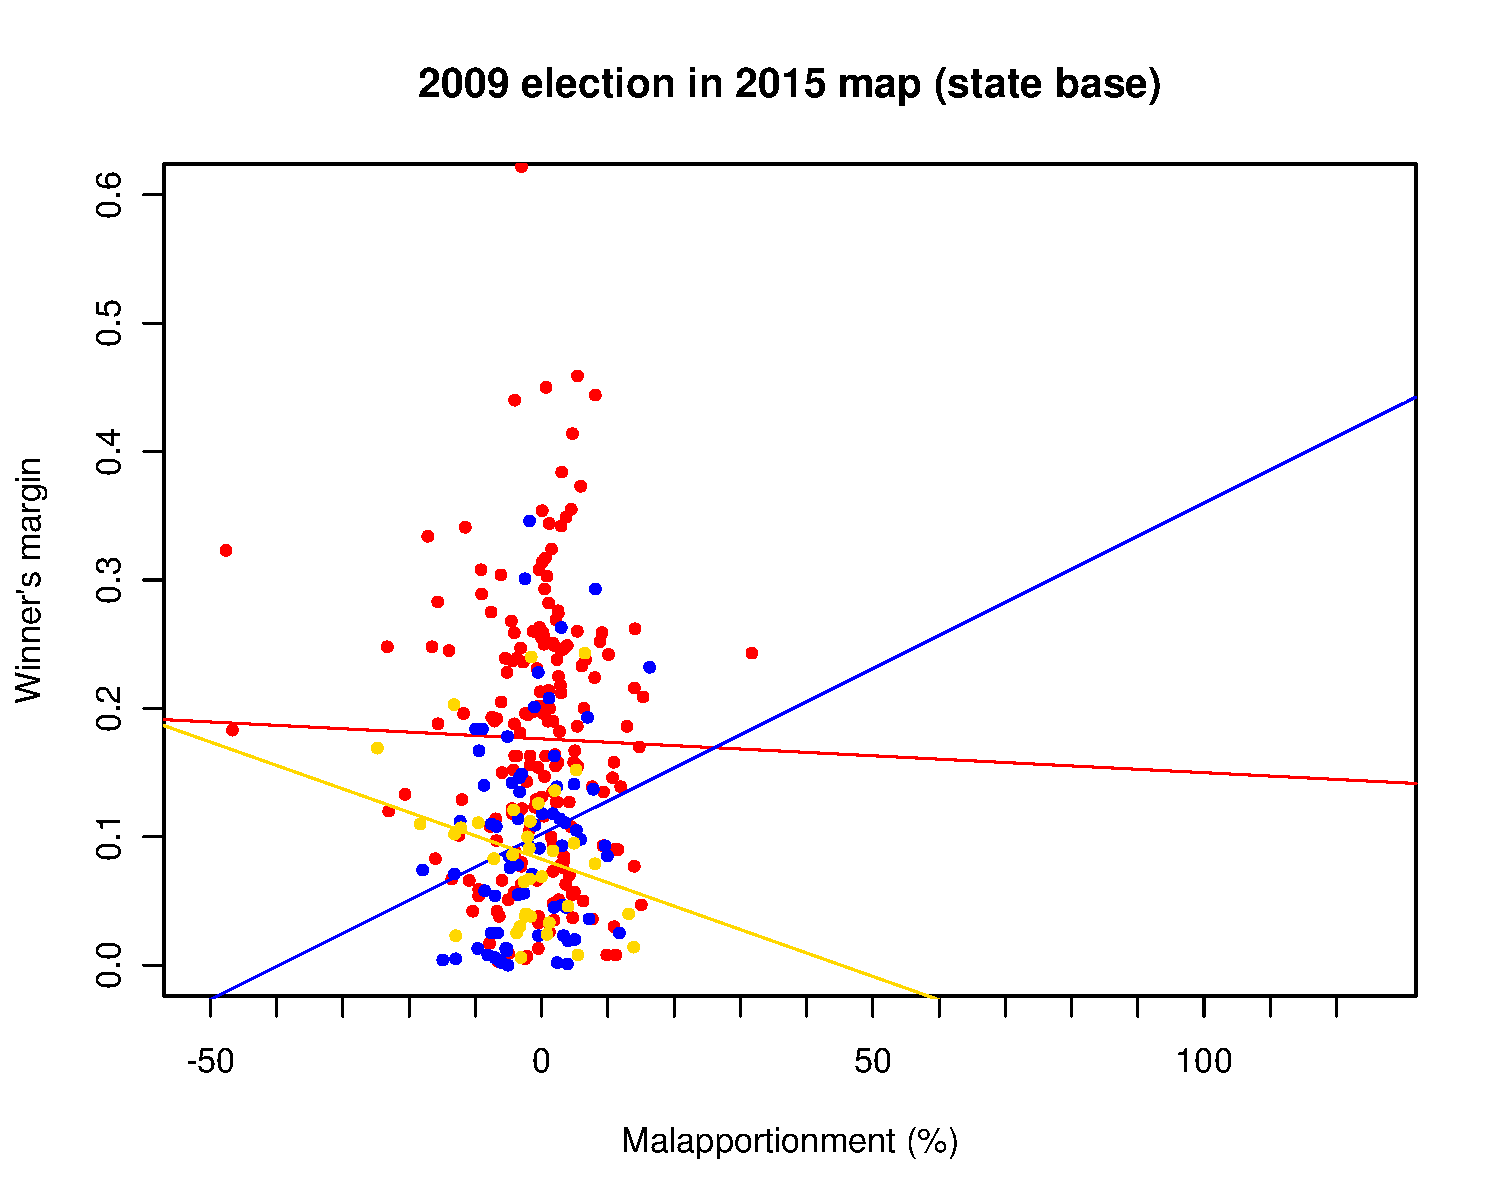
\includegraphics[width=.4\columnwidth]{../graphs/malmg2009d3nat.pdf} \\
    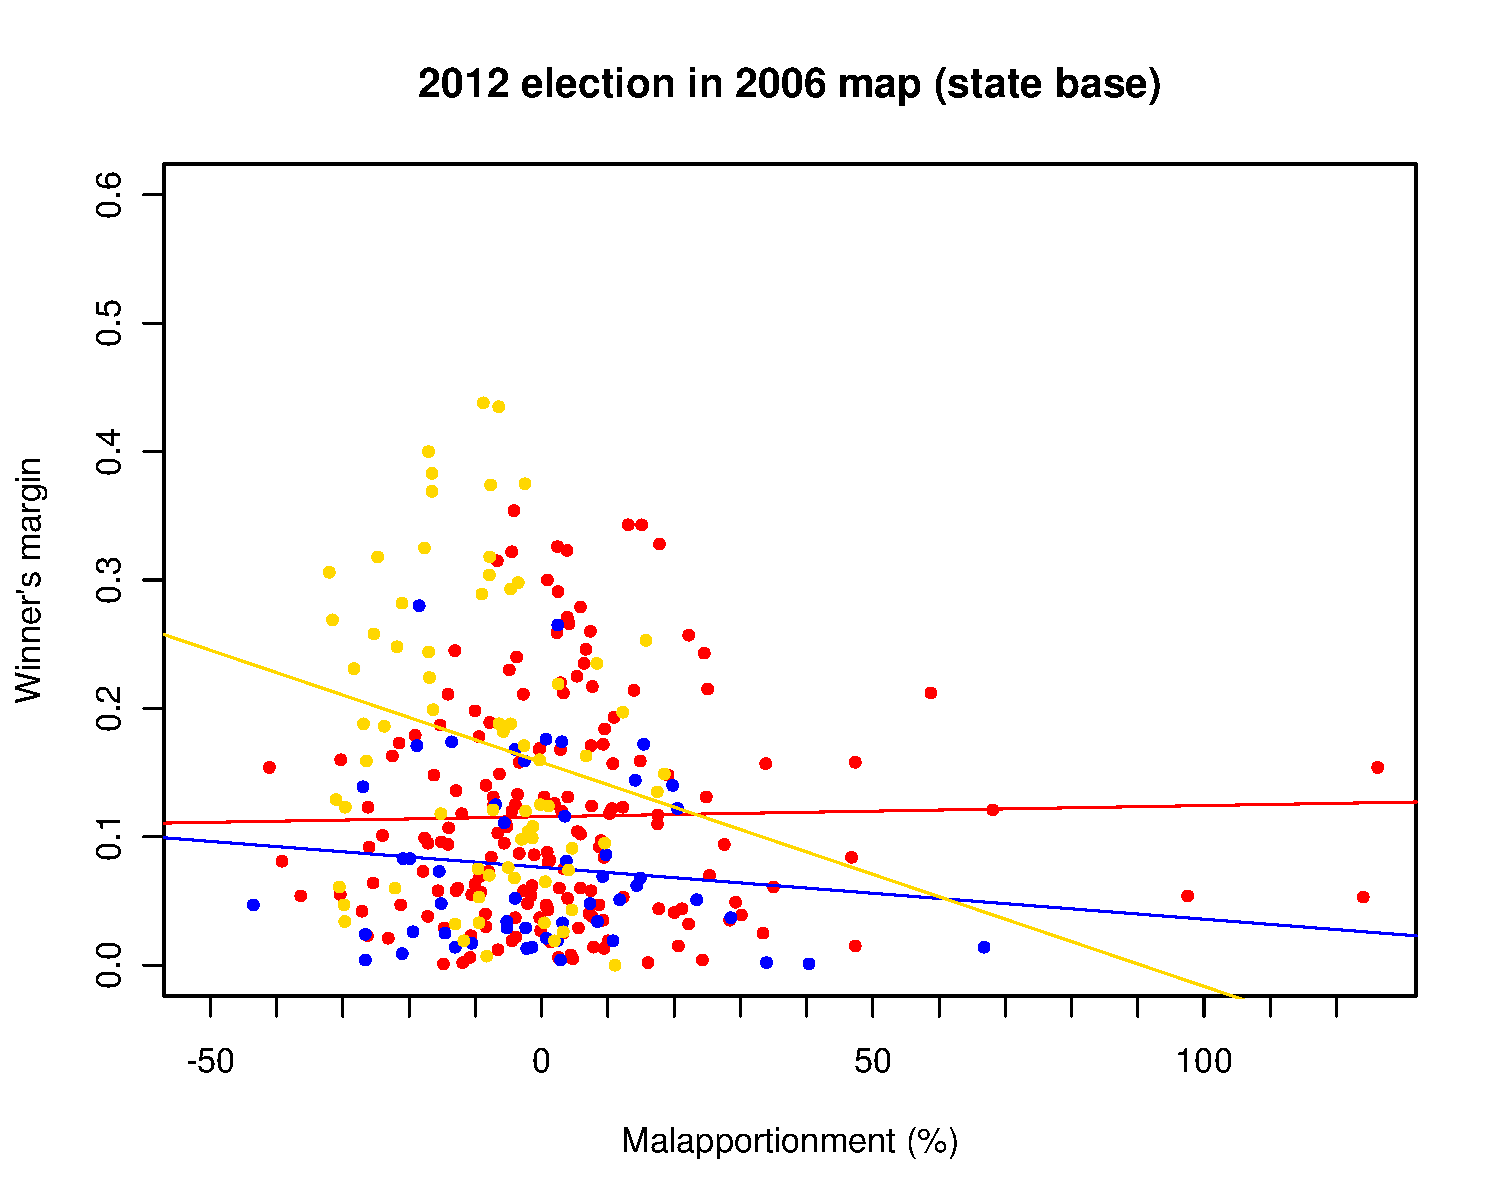
\includegraphics[width=.4\columnwidth]{../graphs/malmg2012d0nat.pdf} & 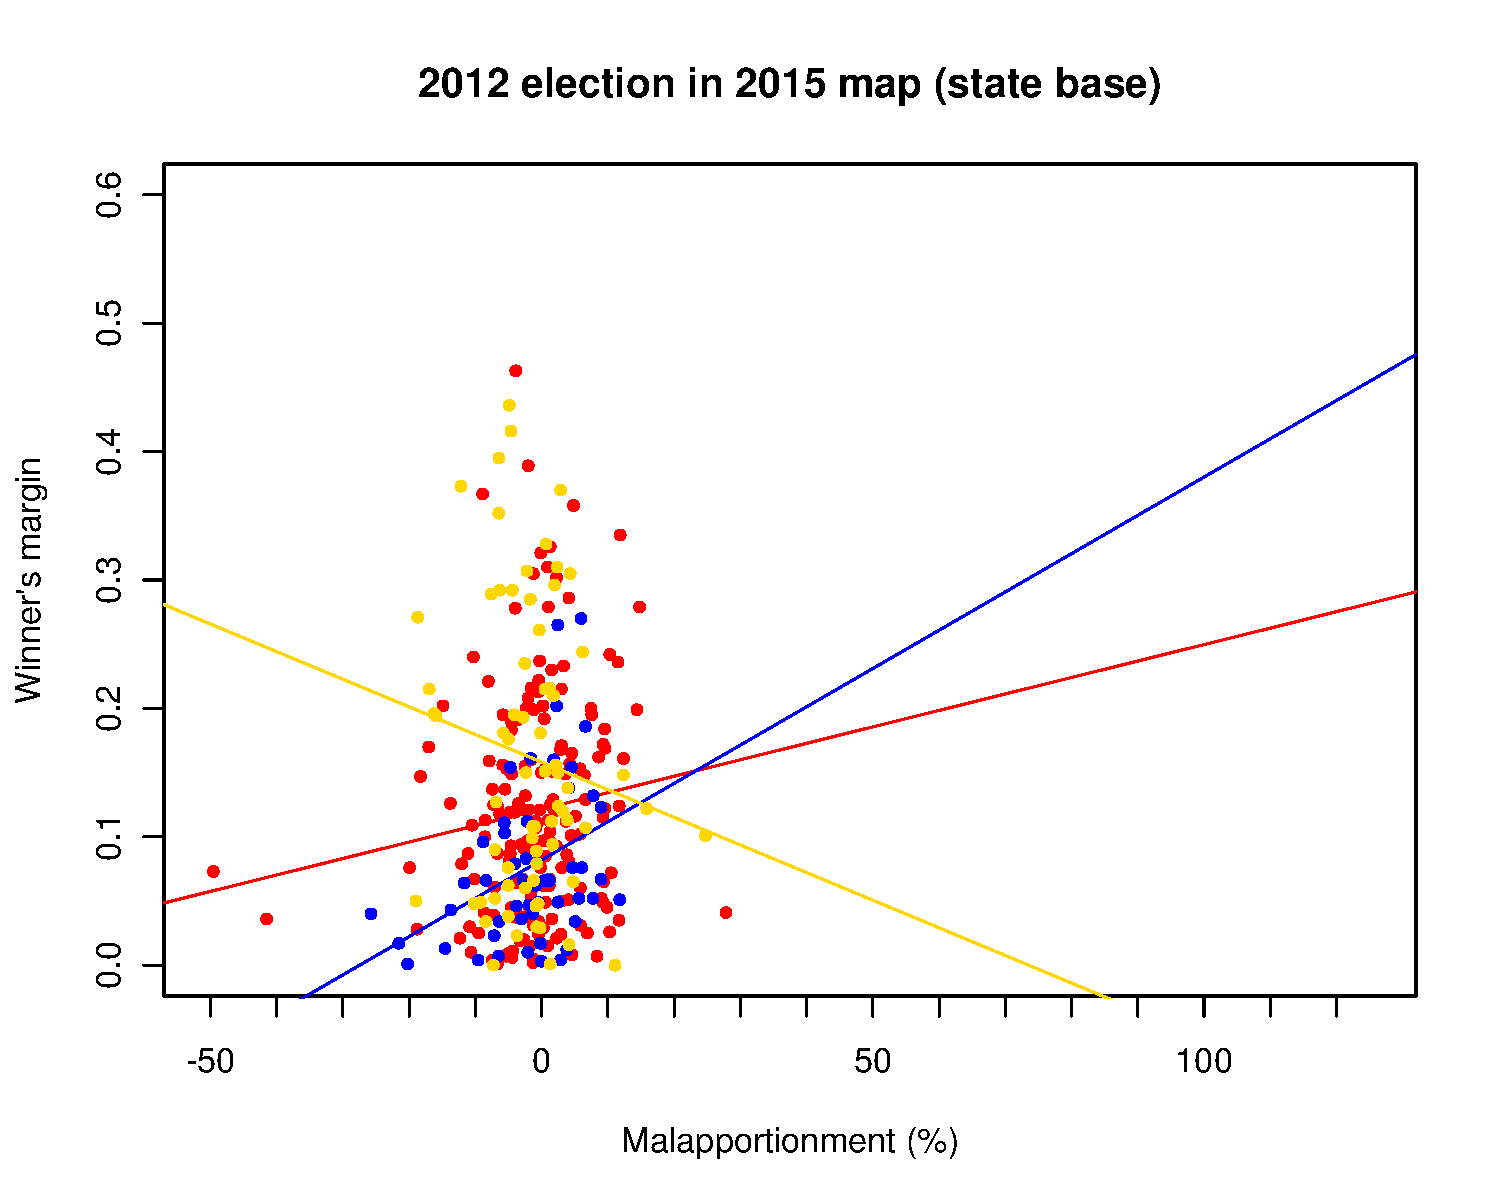
\includegraphics[width=.4\columnwidth]{../graphs/malmg2012d3nat.pdf} \\
  \end{tabular}
  \caption{Vote margin and malapportionment (compared to national average)}\label{F:malmgnat}
\end{center}
\end{figure}

\begin{figure}
\begin{center}
  \begin{tabular}{cc}
    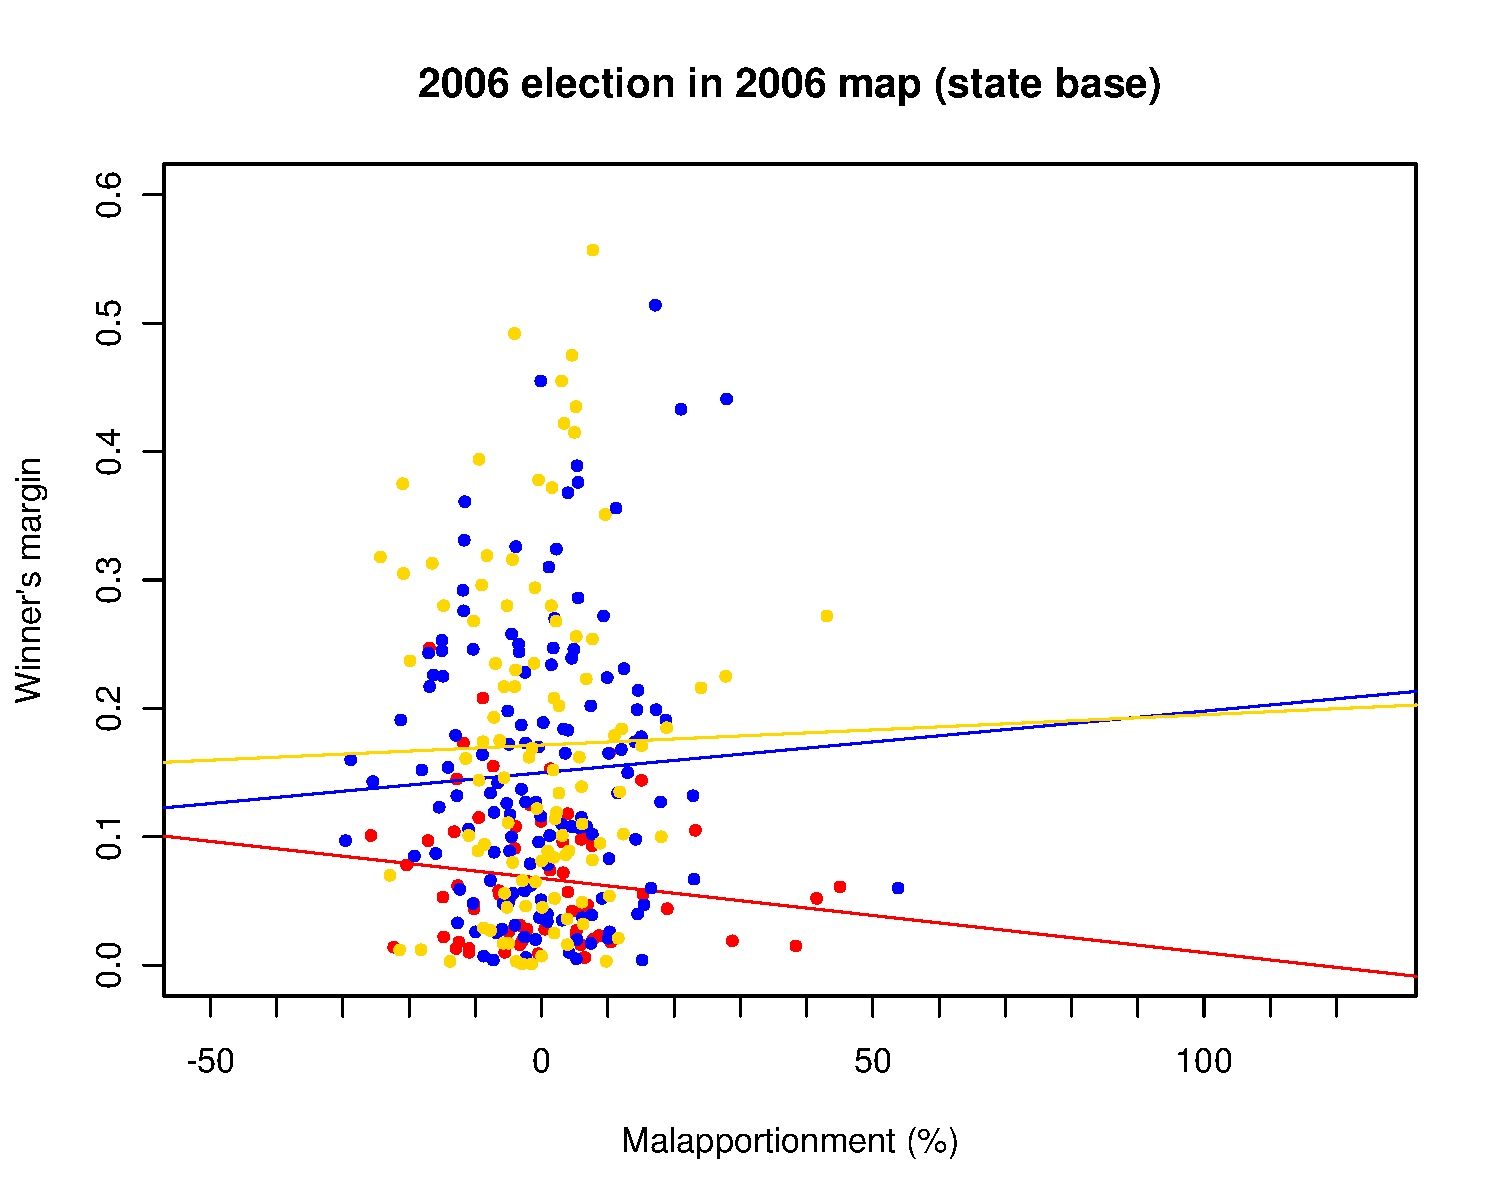
\includegraphics[width=.4\columnwidth]{../graphs/malmg2006d0sta.pdf} & 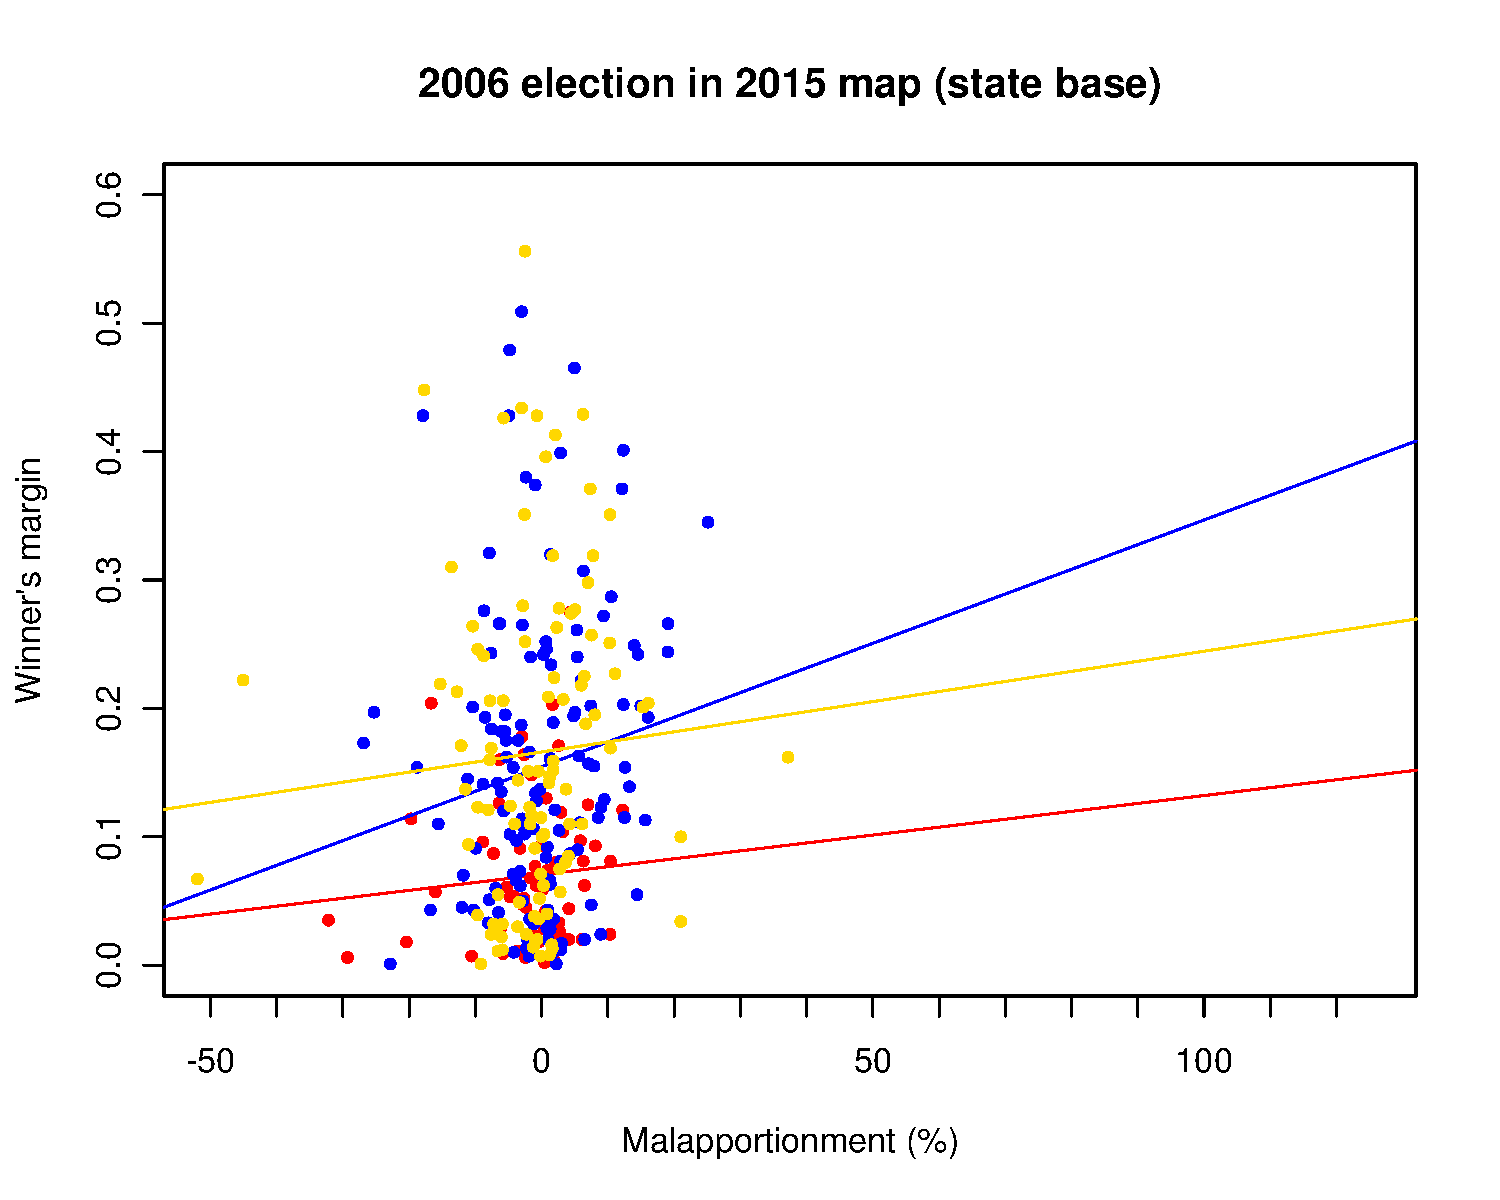
\includegraphics[width=.4\columnwidth]{../graphs/malmg2006d3sta.pdf} \\
    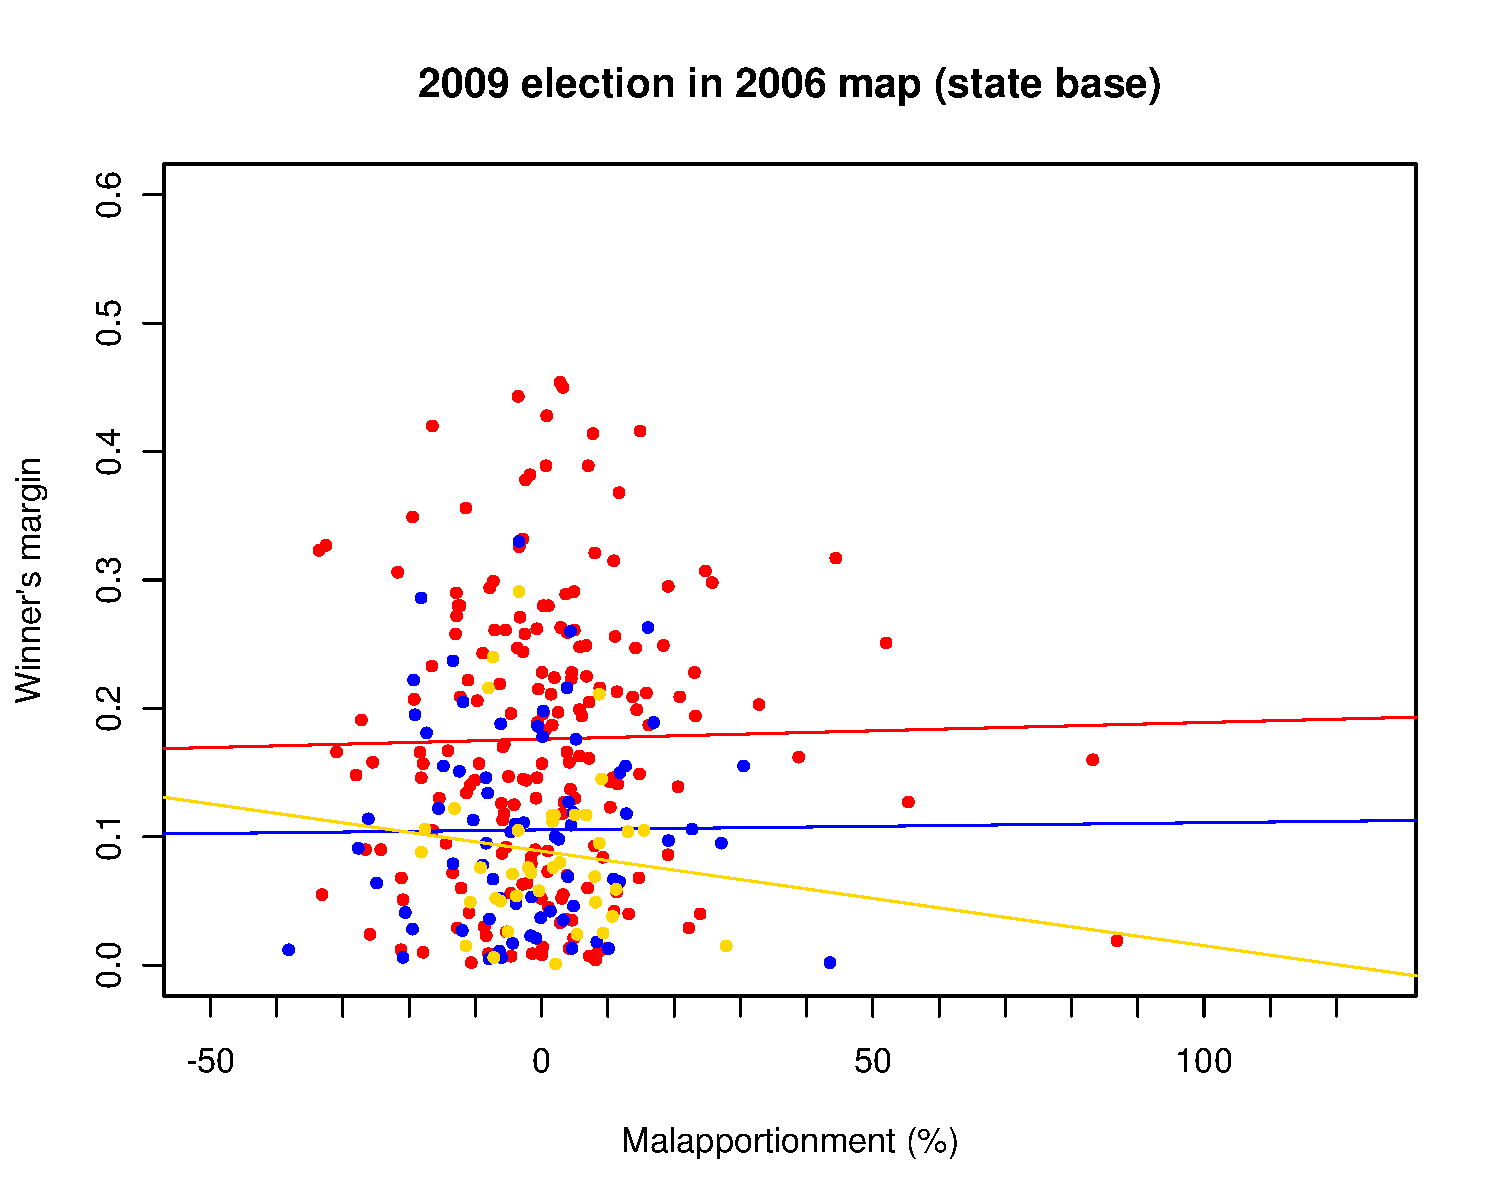
\includegraphics[width=.4\columnwidth]{../graphs/malmg2009d0sta.pdf} & 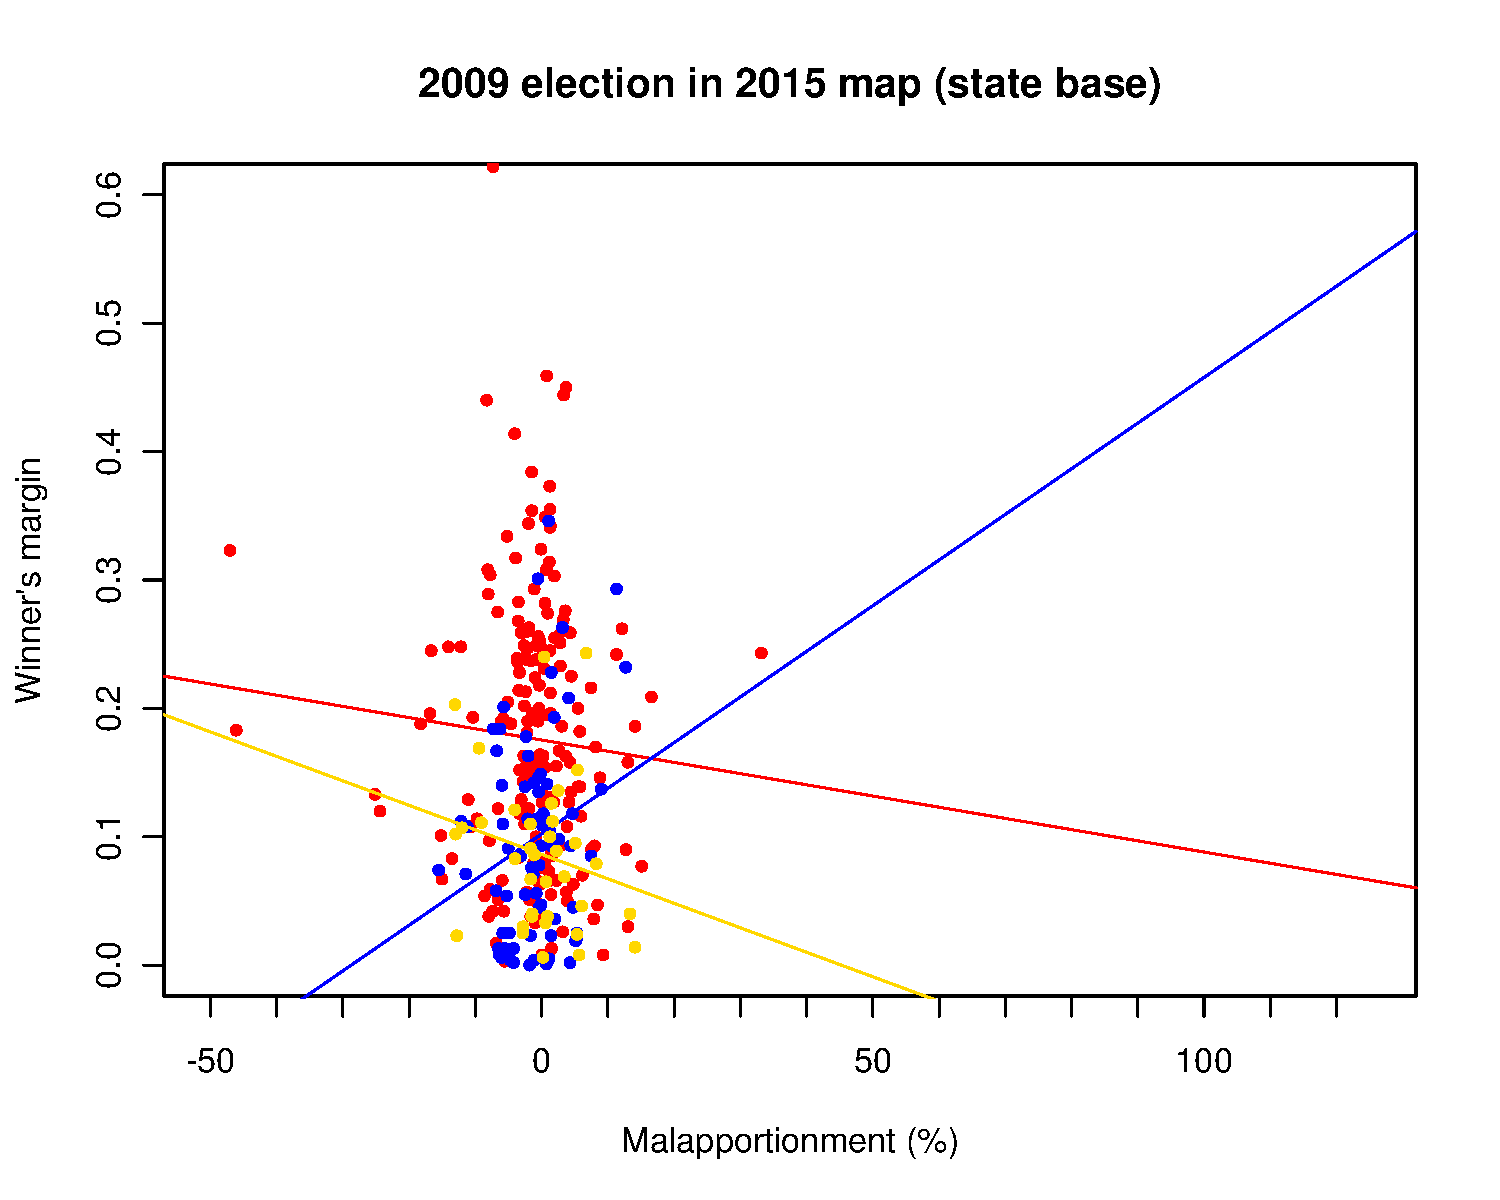
\includegraphics[width=.4\columnwidth]{../graphs/malmg2009d3sta.pdf} \\
    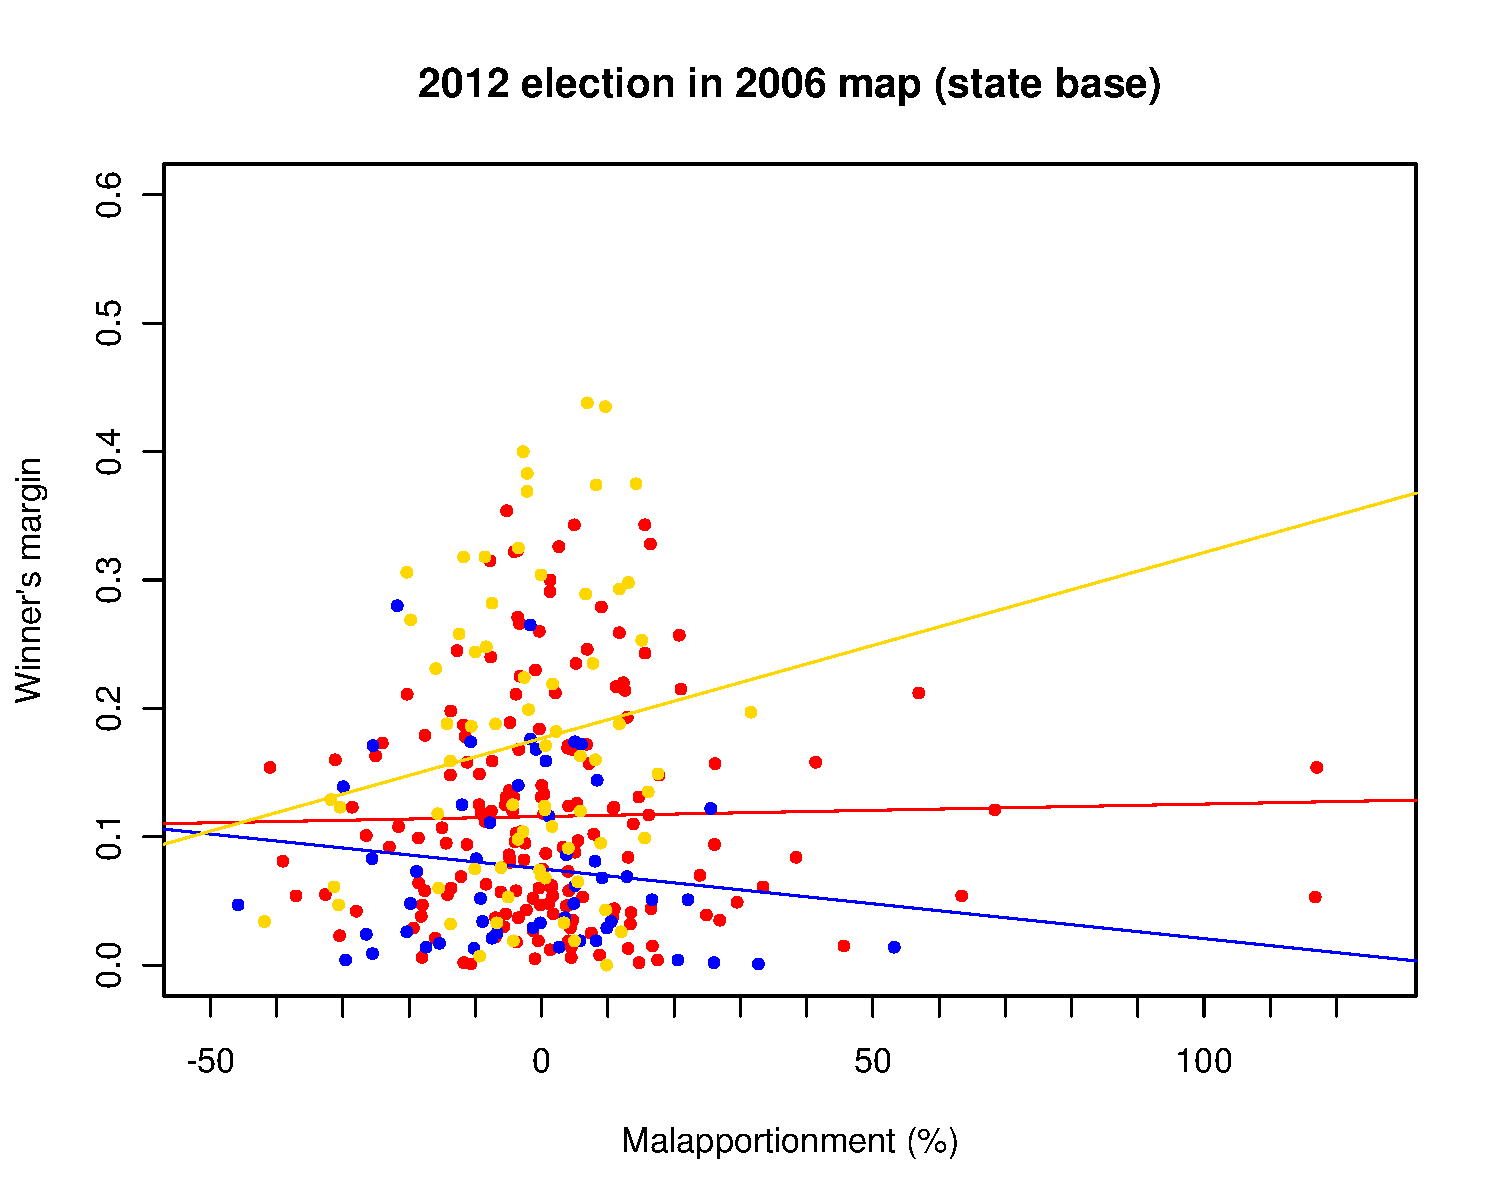
\includegraphics[width=.4\columnwidth]{../graphs/malmg2012d0sta.pdf} & 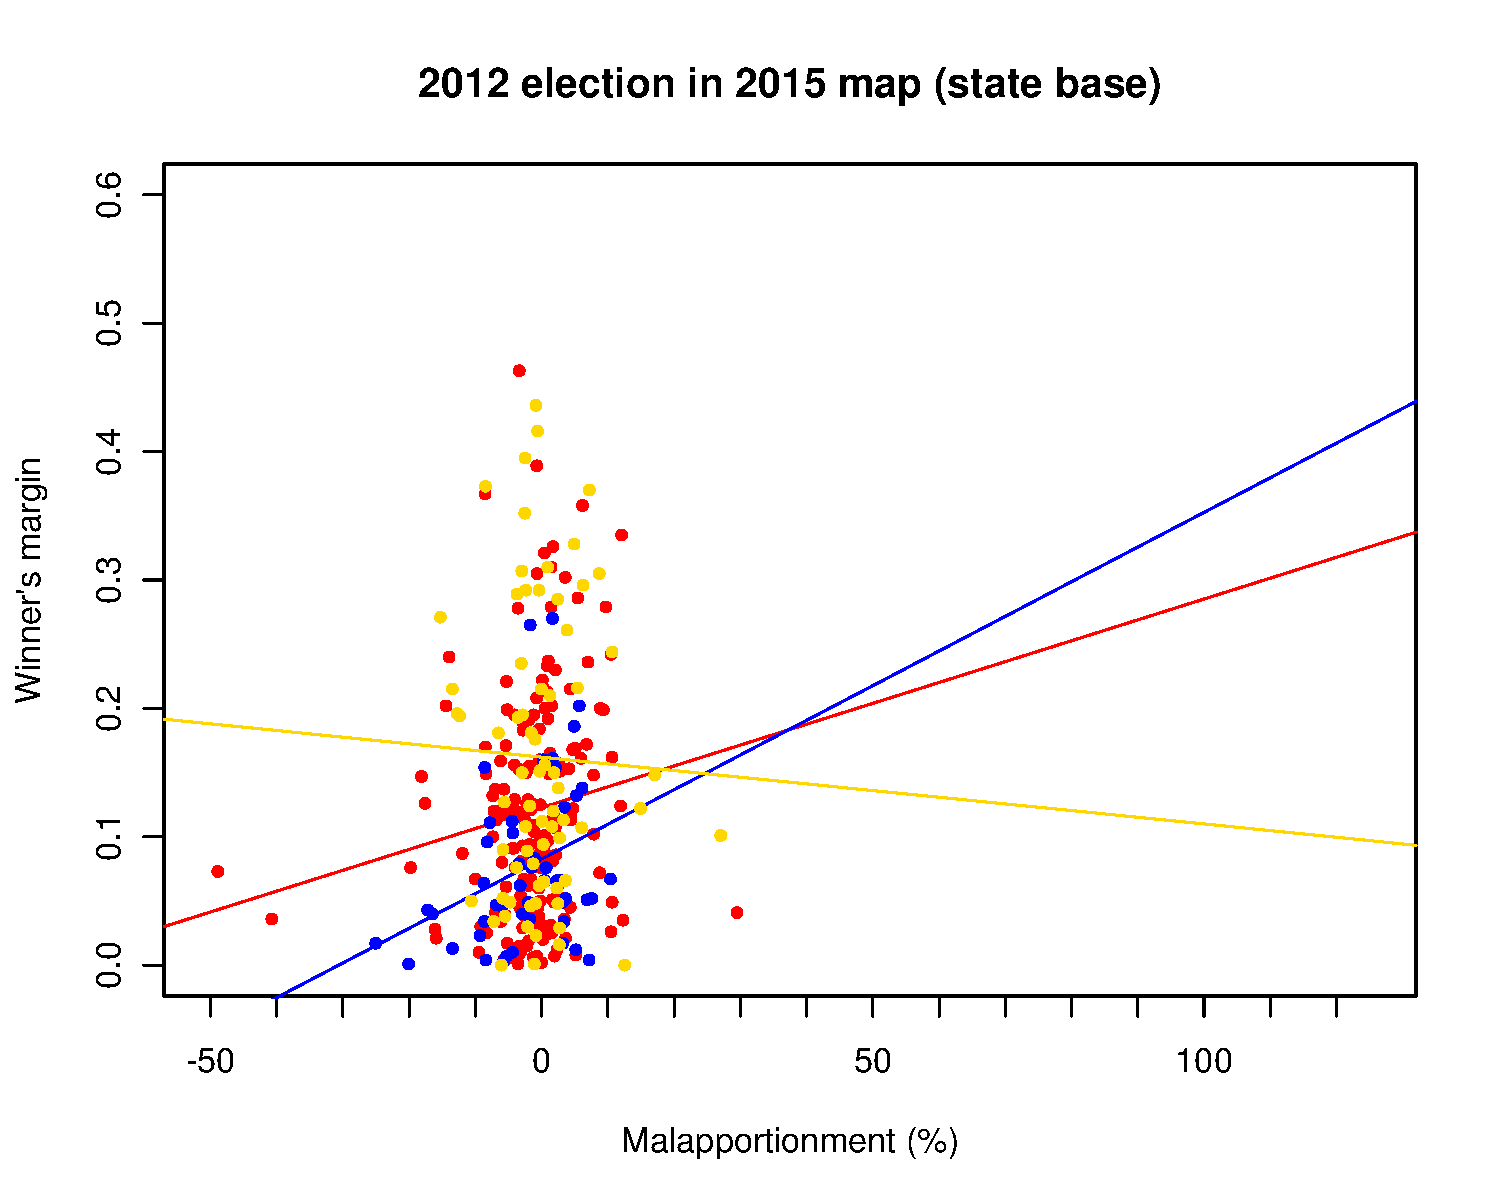
\includegraphics[width=.4\columnwidth]{../graphs/malmg2012d3sta.pdf} \\
  \end{tabular}
  \caption{Vote margin and malapportionment (compared to state averages)}\label{F:malmgnat}
\end{center}
\end{figure}


\section{Elasticity}

One district charateristic is how elastic they are to a party's statewide vote (nationwide?). Elasticity should shape redistricting preferences. A district is highly elastic for the PAN when small shifts in the party's vote statewide correspond to sharp district vote hikes. It is inelastic when it corresponds to more modest district vote changes. Negative elasticity is even conceivable, the district vote growing when the rest of the state shrinks. Local effects on mobilization and voting can move against state effects. If every section in the district is a microcosm of the state's electorate, unit elasticity ensues. 

The measure regresses a party's three-year vote change in the section $\Delta_s$ on the the parent state vote change $\Delta_e$ thus:  

\begin{equation}
\Delta_s = \sum\limits_{d=1}^{D_e} \alpha_d + \beta_d \Delta_e.
\end{equation}

\noindent Fixed effects for each district are considered, fitting separate $\alpha_d$ and $\beta_d$ regression coefficients for every district (indexed $d$). The model is estimated for every state separately because doing it nationwide involves too many sections (67k) and parameters (600) for my machine. 

\begin{figure}
\begin{center}
  \begin{tabular}{cc}
    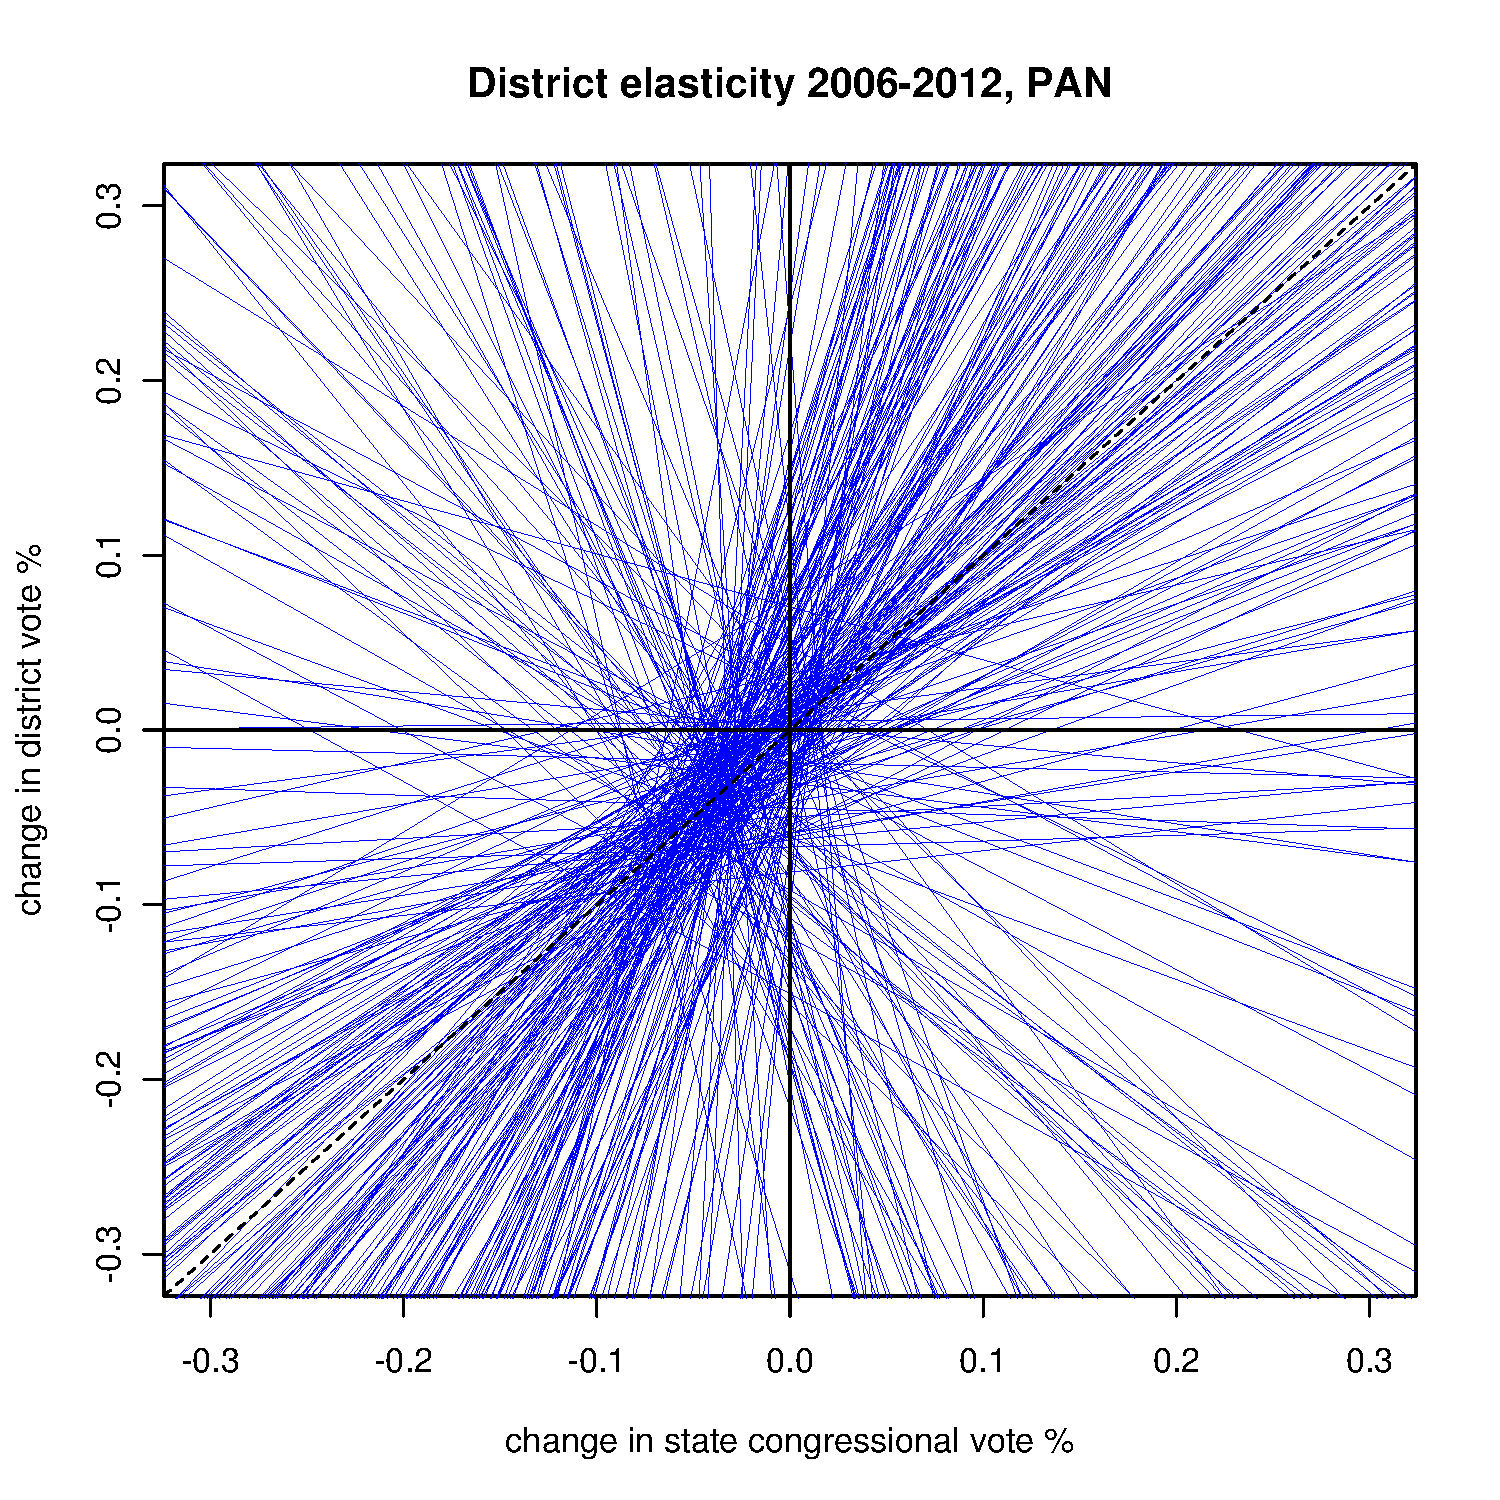
\includegraphics[width=.4\columnwidth]{../graphs/elastpand0.pdf} & 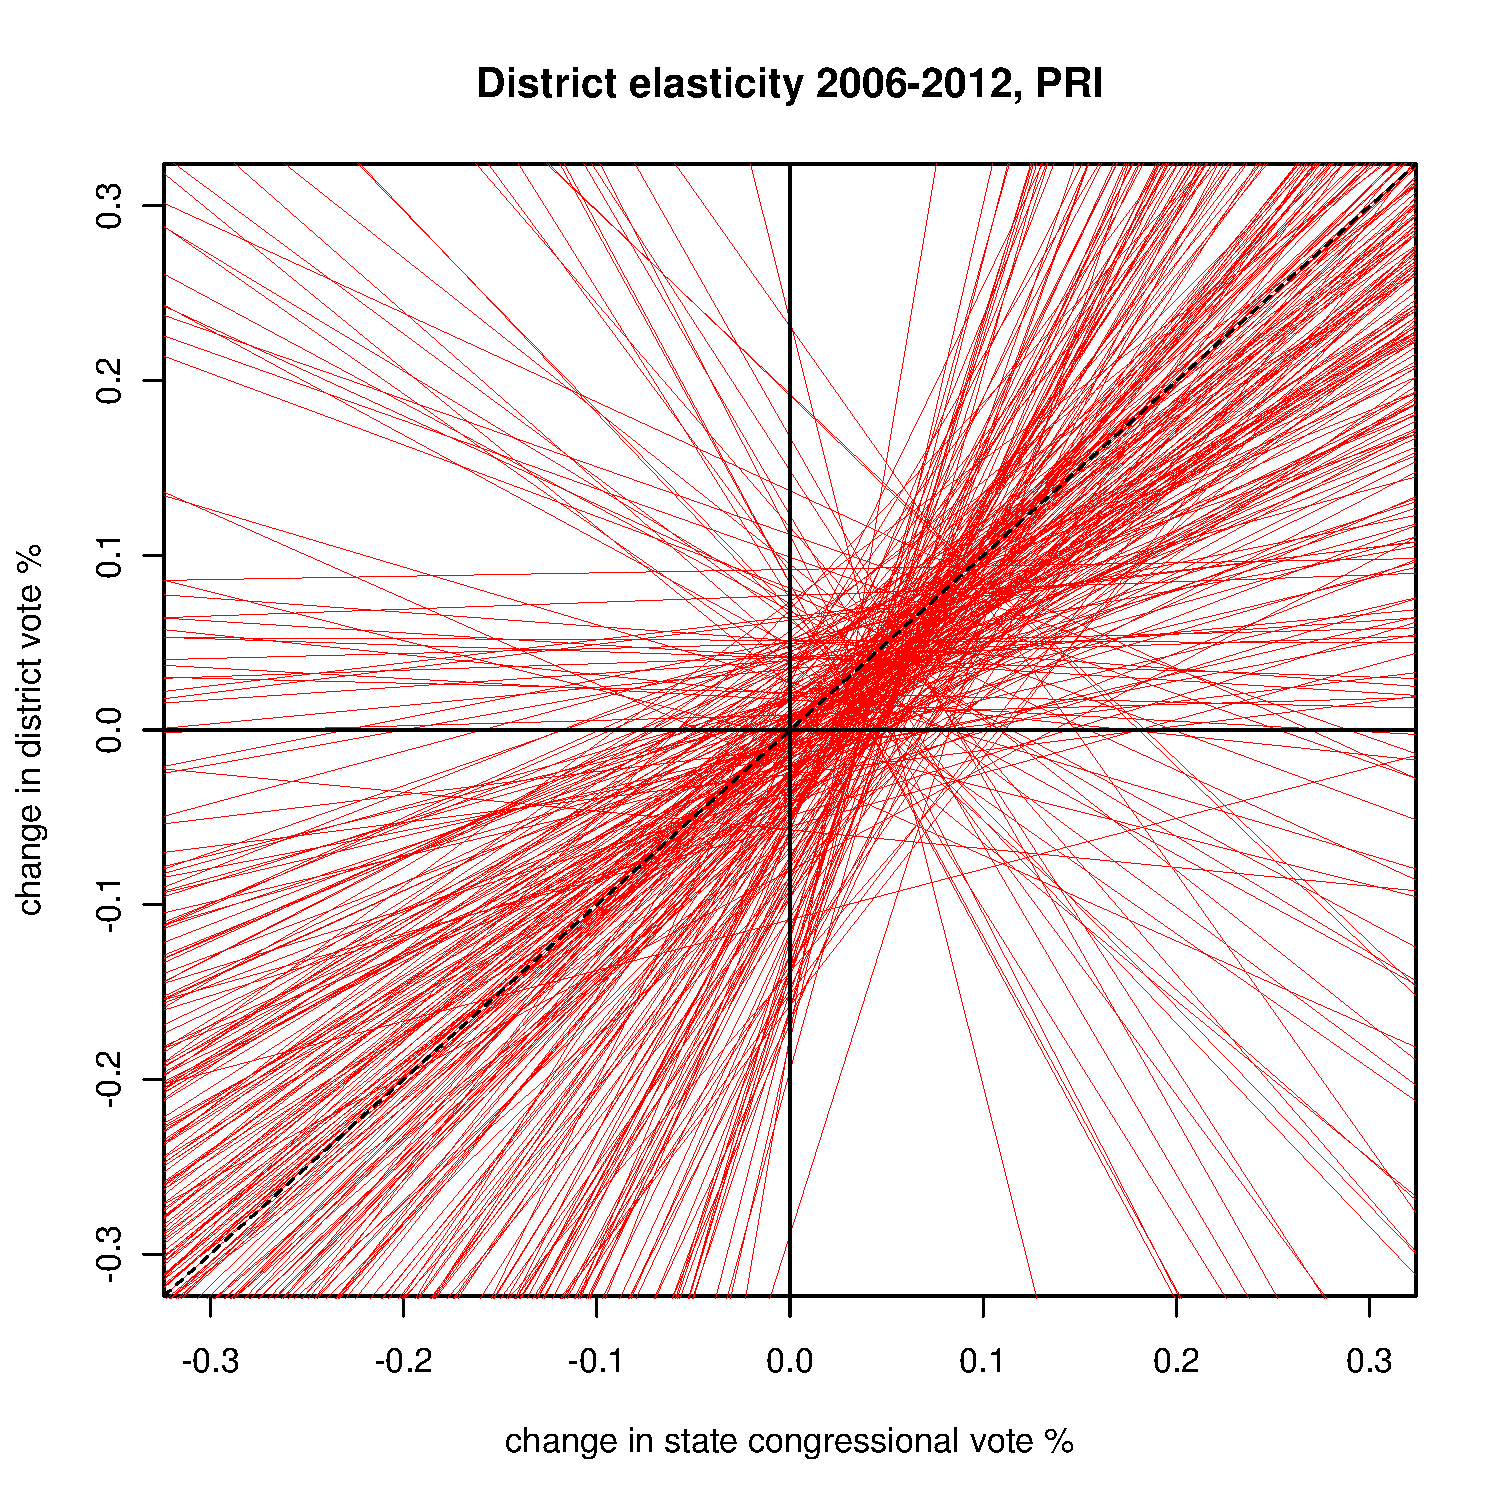
\includegraphics[width=.4\columnwidth]{../graphs/elastprid0.pdf} \\
    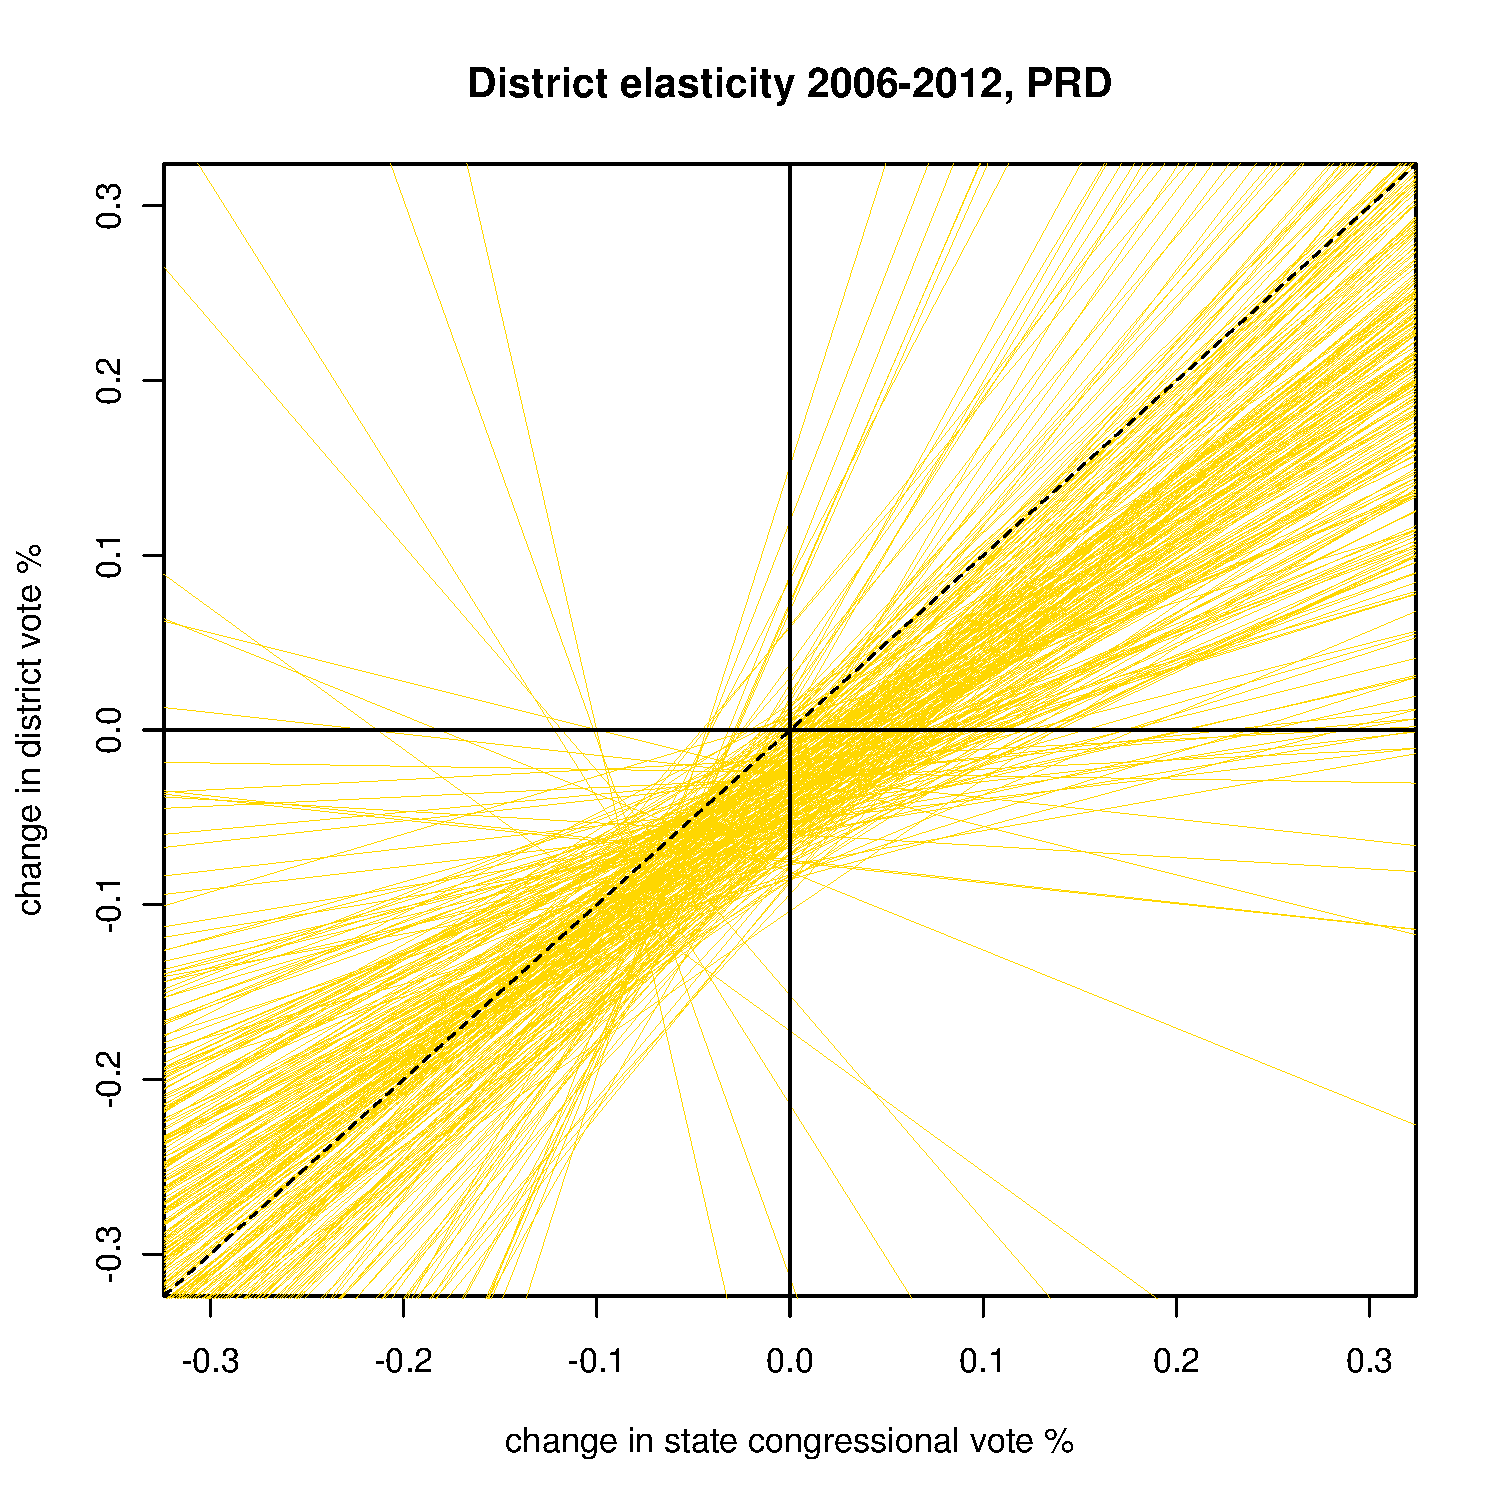
\includegraphics[width=.4\columnwidth]{../graphs/elastprdd0.pdf} &  \\
  \end{tabular}
  \caption{Parties' district elasticities}\label{F:malmgnat}
\end{center}
\end{figure}


sensitive of insulated they are from the party's fate in the state. The measure is associated to the party record \citep{cox.mccubbins.1993}, ``a commonly accepted summary of the past actions, beliefs, and outcomes with which [the party] is associated'' (102). Cox and McCubbins focus on national parties, but recognize that the party record varies from state to state (whose voters focus on different elements of the record). The measure here is how, and how much change in the district vote relates to the statewide change in a party's congressional vote. If every section in the district were a microcosm of the state's electorate, a one-on-one relation would ensue -- a 5 percent drop in the state corresponds to a 5 percent drop in the district. If the party's vote drops less, or even holds or improves, in many of the district's sections, the party performs relatively better (or less badly) in the district. District responsiveness to or insulation from the state party vote may be valuable in different circumstances. 


\section{Conclusion}

Mexico's federal districts exhibit no party bias when analyzed at the state level. Big system responsiveness, typical of first-past-the-post system in units with few federal districts, is associated with the districts. So PRI's tendency to be over-represented more than PAN and PRD, and the PRI's winning of a couple extra seats with the redistricting proposal is not the product of partisan bias. If the PRI wins more this is due to its status as the largest party in more states that the other two major parties combined. 

\section{Alejandro's tables}

Information from Alejandro's first draft should help analyze party feedback to the first and second redistricting proposals. I have merged elements of his first and second tables in Table \ref{T:counterprops}. Could his third table become a crosstabulation of winners vs.\ party?

% \begin{table}
% \begin{center}
%   \begin{tabular}{lrrr|rrr|r}
%     Party & national & local & total 1st & national & local & total 2nd & Total \\ \hline
%     PAN	  & 22 & 20 & 42 & 24 & 16 & 40 & 82 \\
%     PRI	  & 0 & 28 & 28 & 30 & 26 & 56 & 84 \\
%     PRD	  & 27 & 21 & 48 & 29 & 18 & 47 & 95 \\
%     PT	  & 12 & 20 & 32 & 15 & 16 & 31 & 63 \\
%     PVEM  & 0 & 20 & 20 & 28 & 17 & 45 & 65 \\
%     MC    & 17 & 21 & 38 & 32 & 16 & 48 & 86 \\
%     PNA   & 1 & 18 & 19 & 11 & 17 & 28 & 47 \\
%     IFE   & 0 & 9 & 9 & 0 & 13 & 13 & 22 \\ \hline
%     Total & 79 & 157 & 236 & 169 & 139 & 308 & 544 \\
%   \end{tabular}
%   \caption{Counterproposals by party to the first and second scenarios at the National and Local Surveilance Committees. Prepared by authors with information from the Federal Electoral Institute.}\label{T:counterprops}
% \end{center}
% \end{table}
 
\begin{table}
\begin{center}
  \begin{tabular}{lrrr|rrr|r}
    Party & national & local & total 1st & national & local & total 2nd & Total \\ \hline
    PAN	  & 17/22 & 2/20 & 19/42 & 17/24 & 4/16 & 21/40 & 40/82 \\
    PRI	  & 0/0 & 2/28 & 2/28 & 8/30 & 6/26 & 14/56 & 16/84 \\
    PRD	  & 3/27 & 2/21 & 5/48 & 5/29 & 5/18 & 10/47 & 15/95 \\
    PT	  & 1/12 & 1/20 & 2/32 & 3/15 & 1/16 & 4/31 & 6/63 \\
    PVEM  & 0/0 & 1/20 & 1/20 & 7/28 & 3/17 & 10/45 & 11/65 \\
    MC    & 1/17 & 0/21 & 1/38 & 6/32 & 2/16 & 8/48 & 9/86 \\
    PNA   & 0/1 & 1/18 & 1/19 & 4/11 & 3/17 & 7/28 & 8/47 \\
    IFE   & 0/0 & 1/9 & 1/9 & 0/0 & 5/13 & 5/13 & 6/22 \\ \hline
    Total & 22/79 & 10/157 & 32/236 & 50/169 & 29/139 & 43/308 & 111/544 \\
  \end{tabular}
  \caption{Counterproposals to the first and second proposals at the National and Local Surveilance Committees. Denominator reports the number of counterproposals made, numerator how many were adopted. Prepared by authors with information from the Federal Electoral Institute.}\label{T:counterprops}
\end{center}
\end{table}
 
% seats predicted with .33, .33, .33, .005, .005, 0, 0 vote breakdown
%        2.5%     97.5% 
% pan 94.15169 114.54938 
% pri 90.69639 106.57247 
% prd 85.04985 108.23755 

% No hay sistema electoral neutral. Sus partes (los distritos y su magnitud, la presencia de umbrales, la estructura formulaica 
% que traduce votos en esca\~nos, etc.) pueden tener consecuencias distributivas. En particular, lo que interesa aqu\'i es la 
% desproporcionalidad que introduce un plan de redistritaci\'on en la asignaci\'on de esca\~nos. Se suele evaluar la desproporcionalidad 
% en relaci\'on a la representaci\'on proporcional ideal---aqu\'ella que asignar\'ia exactamente 13.5 por ciento de diputados al partido 
% que obtuviese 13.5 por ciento del voto. M\'as generalmente, en el tipo ideal de referencia se espera que la relaci\'on entre votos y 
% esca\~nos siga la l\'inea diagonal punteada en el croquis siguiente. Un partido sobrerrepresentado aparecer\'ia sesgado a la 
% izquierda de la diagonal (obtiene igual porcentaje de esca\~nos con menos votos), uno subrepresentado sesgado a la derecha. 

\bibliographystyle{apsr}
%\bibliography{d:/01/mydocs/magar}
\bibliography{../../../../../mydocs/magar}


\end{document}
